\documentclass{article}
\usepackage{iclr2026_conference,times}

\input{math_commands.tex}

\usepackage{amsmath,amssymb,amsthm,mathtools}
\usepackage{algorithm}
\usepackage{algorithmic}
\usepackage{booktabs}
\usepackage{enumitem}
\usepackage{graphicx}
\usepackage{microtype}
\usepackage{tikz}
\usetikzlibrary{calc}
\usepackage{xcolor}
\usepackage{url}
\usepackage{hyperref}
\hypersetup{
  colorlinks=true,
  linkcolor=blue,
  citecolor=blue,
  urlcolor=blue
}

\newtheorem{theorem}{Theorem}
\newtheorem{lemma}[theorem]{Lemma}
\newtheorem{proposition}[theorem]{Proposition}
\newtheorem{corollary}[theorem]{Corollary}
\newtheorem{definition}[theorem]{Definition}
\newtheorem{remark}[theorem]{Remark}
\newtheorem{assumption}{Assumption}

\providecommand{\argmax}{\mathop{\mathrm{arg\,max}}\limits}
\providecommand{\argmin}{\mathop{\mathrm{arg\,min}}\limits}

\title{Buffered ERM for Finite-Generation\\LLM Ensembles}
\author{Anonymous Authors}

% Uncomment only for a camera-ready version.
% \iclrfinalcopy

\begin{document}
\maketitle

\begin{abstract}
Weighted aggregation of frozen large language models is often analyzed as if
each model's answer distribution were known.  A deployed ensemble instead sees
empirical answer frequencies from finitely many generations.  This creates two
independent sample sizes: \(Q\) labeled questions used to learn the ensemble
weights and \(N\) generations used to estimate each model's answer distribution
on each labeled training question.  Raw empirical risk minimization can exploit
sign errors near ties.  We study a margin-buffered estimator that counts a
training question as solved only when the empirical gold-answer margin exceeds
its finite-generation uncertainty radius.  Under a one-sided margin condition
at the best fixed weight, the clean population excess risk of the learned
weights is the sum of a standard
\(Q^{-1/2}\) generalization term and an
\(N^{-\beta/2}\) boundary-resolution term, up to logarithmic factors.  A
hard-margin two-point construction shows that a margin condition alone cannot
improve the \(Q\)-rate.  Faster \(Q\)-rates become available only after adding
identifiable risk growth and an absolute margin condition.  We give a direct
MILP implementation, preserve reproducible finite-generation diagnostics from
the earlier system, and state separately the benchmark experiment still needed
to evaluate the calibrated buffer itself.
\end{abstract}

\section{Introduction}
\label{sec:intro}

Repeated sampling has become a standard test-time tool for language models.
Self-consistency aggregates multiple reasoning paths, best-of-\(N\) procedures
select among sampled candidates, and multi-model systems combine complementary
models or agents \citep{wang2022selfconsistencyic,brown2024largelm,
jiang2023llmblenderel,wang2024mixtureofagentsel}.  These methods turn inference
compute into improved answer coverage, but they also make the statistical unit
of observation easy to blur.  An ensemble is evaluated across questions, while
the score used on any one question is itself estimated from repeated
generations.

We study this distinction for convex weighting of \(K\) frozen language
models, following the Best-of-Infinity setting of
\citet{komiyama2026best}.  Each model induces an unknown distribution over the
candidate answers to a question.  If those distributions were known, learning
the weight vector would be an ordinary supervised aggregation problem.  In
practice, the distribution of each model is replaced by vote frequencies from
\(N\) generations, and the weights are selected from \(Q\) labeled questions.
The resulting procedure has two independent sources of error: generalization
from \(Q\) questions and Monte Carlo error from \(N\) generations per model and
training question.

The second source is not merely another smooth estimation term.  Correctness is
determined by the sign of the smallest gold-versus-contender score gap.  A small
perturbation is harmless on a well-separated training question but can reverse
its empirical status near a tie.  Worse, raw empirical risk minimization
searches over weights using those noisy signs, so it can select a weight vector
that benefits from finite-\(N\) errors.  This is a structured instance of
selection under noisy estimates \citep{smith2006theoc}.

Our response is deliberately simple.  Instead of crediting every positive
empirical margin, buffered ERM credits a training question only when its margin
exceeds a uniform finite-generation radius
\(\varepsilon_N(\delta)=\sqrt{2\log(8KAQ/\delta)/N}\), where \(A\) bounds the
number of candidate answers.  Uniform concentration then places the noisy
buffered loss between two clean losses: the ordinary zero-threshold loss and a
clean loss with threshold \(2\varepsilon_N\).  This sandwich compares the
learned weights with one fixed population comparator and avoids imposing a
margin assumption at the random estimator.

Under the one-sided condition
\(\Pr\{0<M_q(w^\star)\le t\}\le C_m t^\beta\), the resulting excess-risk bound
is
\begin{equation}
R(\widehat w_\varepsilon)-R(w^\star)
\lesssim
\sqrt{\frac{(K-1)\log(eAQ)+\log(1/\delta)}{Q}}
+
C_m\left(\frac{\log(KAQ/\delta)}{N}\right)^{\beta/2}.
\label{eq:intro-rate}
\end{equation}
The first term is standard generalization over questions.  The second is the
mass of comparator-correct training questions that cannot be distinguished
from ties at resolution \(N^{-1/2}\).  It can decay faster than \(N^{-1/2}\)
because the target is a thresholded decision, not estimation of a smooth
probability.  Equation~\ref{eq:intro-rate} concerns the clean population risk
of the learned weights.  If deployment also uses finitely many fresh
generations, prediction-time sign errors form an additional term; we state the
available fixed-weight guarantee in Appendix~\ref{app:legacy-support} rather
than hiding it inside the main theorem.

The same margin exponent does \emph{not} automatically accelerate the
\(Q\)-term.  We give a two-model construction with margins of magnitude one at
each optimum, yet deciding which separated region of the simplex is better
reduces to distinguishing two nearly fair coins.  Its minimax excess risk is
of order \(Q^{-1/2}\).  This isolates the missing ingredient: a boundary
condition controls local disagreement, while a fast learning rate also needs
global identifiability.  We therefore state the faster result only under an
absolute margin condition together with local risk growth and global
separation.

Our contributions are:
\begin{enumerate}[leftmargin=*,itemsep=2pt,topsep=3pt]
\item We formulate finite-generation LLM weighting as a two-sample-size
problem and introduce a margin-buffered ERM with a direct mixed-integer linear
implementation.
\item We prove the robust bound in Eq.~(\ref{eq:intro-rate}) using only a
one-sided margin condition at the best fixed weight.
\item We prove that hard margins alone do not imply a fast \(Q\)-rate, then
derive an optional localized rate under explicit geometric identifiability.
\item We separate verified legacy diagnostics from direct evidence for the new
estimator and specify the artifact-complete experiment required to close that
gap.
\end{enumerate}

\section{Related Work}
\label{sec:related}

\paragraph{Test-time sampling and LLM ensembles.}
Self-consistency made majority aggregation of sampled reasoning paths a common
inference primitive \citep{wang2022selfconsistencyic}.  Repeated-sampling and
test-time scaling studies characterize how coverage and accuracy change with
additional inference compute \citep{brown2024largelm,schaeffer2025howdl,
snell2025scalinglt,wu2024inferencesl}.  Multi-model systems instead exploit
variation across frozen models, using ranking and fusion or layered agent
aggregation \citep{jiang2023llmblenderel,wang2024mixtureofagentsel}.
\citet{komiyama2026best} study the population, or best-of-infinity, limit of
weighted test-time ensembling.  Our question is complementary: what guarantee
survives when each population answer distribution is represented by only
\(N\) generations and the weights are fitted on only \(Q\) questions?

\paragraph{Aggregation of fixed predictors.}
Linear opinion pools and forecast combinations have a long history
\citep{stone1961opinionpool,bates1969combination,genest1986combining}.
Stacking learns how to combine fixed predictors
\citep{wolpert1992stacked,breiman1996stacked}, while weighted-majority methods
study adaptive combinations of experts \citep{littlestone1994weighted}.  Our
predictor is a linear opinion pool over answer distributions, followed by an
\(\arg\max\).  The question-dependent candidate set changes the geometry, but
on a fixed sample the relevant labelings are still induced by an arrangement
of affine hyperplanes in the weight simplex.

\paragraph{Margins, capacity, and fast rates.}
Margin distributions are central to the analysis of voting classifiers
\citep{schapire1997boostingtm,koltchinskii2001furthereo}.  VC growth bounds give
the baseline uniform deviation over questions
\citep{vapnik1971uniform,blumer1989learnability}, and Hoeffding concentration
controls the empirical answer frequencies \citep{hoeffding1963probability}.
Low-noise and margin assumptions can yield fast classification and aggregation
rates when paired with suitable localization or curvature
\citep{mammen1999smooth,tsybakov2004optimal,massart2006risk,
bartlett2005local,koltchinskii2006local,audibert2005fastlr}.  Our negative
example matters precisely here: boundary mass at an optimum does not rule out
a nearly tied, well-separated competing optimum.  The optional fast theorem
therefore derives its Bernstein condition from both absolute boundary control
and explicit risk growth, rather than attributing the faster rate to the margin
condition alone.

\paragraph{Certificates and diagnostics.}
PAC--Bayes analyses provide useful diagnostics for distributions over
predictors \citep{mcallester1999pacbayes,dziugaite2017computing}, and specialized
results connect Gibbs and majority-vote risks
\citep{viallard2021selfboundingmv,wu2021chebyshevcantellipi}.  The retained
PAC--Bayes numbers in this project are contextual diagnostics; they are not the
certificate proved here.  Our main argument instead uses a deterministic
buffered predictor, finite-sample margin concentration, and a clean
indicator-sandwich comparison.

\section{Method}
\label{sec:method}

\subsection{Two samples behind one ensemble}
\label{sec:method-setup}

There are \(K\) frozen language models, indexed by \(i=1,\ldots,K\).
Problems are drawn independently from an unknown distribution \(\mathcal D\);
the labeled training benchmark is \(q_1,\ldots,q_Q\).  Each problem \(q\) has a
finite candidate set \(\mathcal A(q)\), with
\(|\mathcal A(q)|\le A\), and gold answer \(a^\star(q)\).
Model \(i\) induces an answer distribution \(p_i(\cdot\mid q)\).  We do not
observe that distribution.  Instead, we draw \(N\) independent generations
\(Y_{i,1}(q),\ldots,Y_{i,N}(q)\) and form
\begin{equation}
\widehat p_i(a\mid q)
=
\frac1N\sum_{n=1}^N\mathbf 1\{Y_{i,n}(q)=a\}.
\label{eq:phat}
\end{equation}
Thus \(\widehat p_i(a\mid q)\) is simply a normalized vote count.  The vectors
\(p_i(\cdot\mid q)\) and \(\widehat p_i(\cdot\mid q)\) lie in the probability
simplex over \(\mathcal A(q)\): they have one nonnegative coordinate per answer
and their coordinates sum to one.  This construction exposes two independent
sample sizes.  \(Q\) controls learning across problems; \(N\) controls how well
each model's answer distribution is measured on a problem.

An ensemble uses a convex weight vector
\(w\in\Delta_K=\{w\in\mathbb R_+^K:\sum_iw_i=1\}\).  It assigns answer \(a\)
the population and empirical scores
\begin{equation}
s_q(a;w)=\sum_{i=1}^K w_i p_i(a\mid q),
\qquad
\widehat s_q(a;w)=\sum_{i=1}^K w_i\widehat p_i(a\mid q).
\label{eq:scores}
\end{equation}
The corresponding predictors return the highest-scoring answer.  Equal
weights recover ordinary voting; nonuniform weights give a weighted plurality
vote.  In the large-\(N\) limit, empirical voting converges to
\(\arg\max_a s_q(a;w)\).

\subsection{The hardest contender determines correctness}
\label{sec:method-margin}

For each wrong answer \(a\ne a^\star(q)\), define the \(K\)-vector
\(\Delta_{q,a}=p_\cdot(a^\star(q)\mid q)-p_\cdot(a\mid q)\), and define
\(\widehat\Delta_{q,a}\) analogously.  The inner product
\(\langle w,\Delta_{q,a}\rangle\) is the ensemble score of the gold answer
minus the score of \(a\).  It is positive when the gold answer beats that
contender and negative when the contender wins.  Because a correct prediction
must beat every wrong answer, the relevant margin is the smallest such gap:
\begin{equation}
M_q(w)=\min_{a\ne a^\star(q)}\langle w,\Delta_{q,a}\rangle,
\qquad
\widehat M_q(w)=
\min_{a\ne a^\star(q)}
\langle w,\widehat\Delta_{q,a}\rangle.
\label{eq:margins}
\end{equation}
Taking the minimum is conservative, not favorable: it selects the hardest
wrong answer.  Hence \(M_q(w)>0\) means that every gap is positive and the
ensemble is correct; \(M_q(w)\le0\) means that some wrong answer ties or wins.
We count ties as errors and write
\begin{equation}
\ell_q(w)=\mathbf 1\{M_q(w)\le0\},
\qquad
R(w)=\mathbb P_{q\sim\mathcal D}\{M_q(w)\le0\}.
\label{eq:risk}
\end{equation}

For a concrete example, consider two models and two wrong answers with
\(\Delta_{q,a_1}=(0.4,-0.1)\), \(\Delta_{q,a_2}=(0.1,0.3)\), and
\(w=(0.5,0.5)\).  The two gaps are \(0.15\) and \(0.20\), so the margin is
\(0.15>0\): the ensemble is correct, and \(a_1\) is the binding contender.

The same definition has a useful geometric reading.  With one wrong answer,
the correct weights form one halfspace of the \((K-1)\)-dimensional weight
simplex.  With several wrong answers, correctness requires all corresponding
halfspace inequalities.  Its closure is therefore a polytope, and the strict
correct region is the relative interior selected by those inequalities.
Across \(Q\) problems, at most \(Q(A-1)\) such hyperplanes partition the
simplex.  This is why the statistical complexity depends primarily on the
weight dimension \(K-1\), with only logarithmic dependence on the number of
contenders in the finite-sample arrangement bound.  Figure~\ref{fig:weight-geometry}
restores the geometric view developed in the reviewed draft.

\begin{figure}[t]
\centering
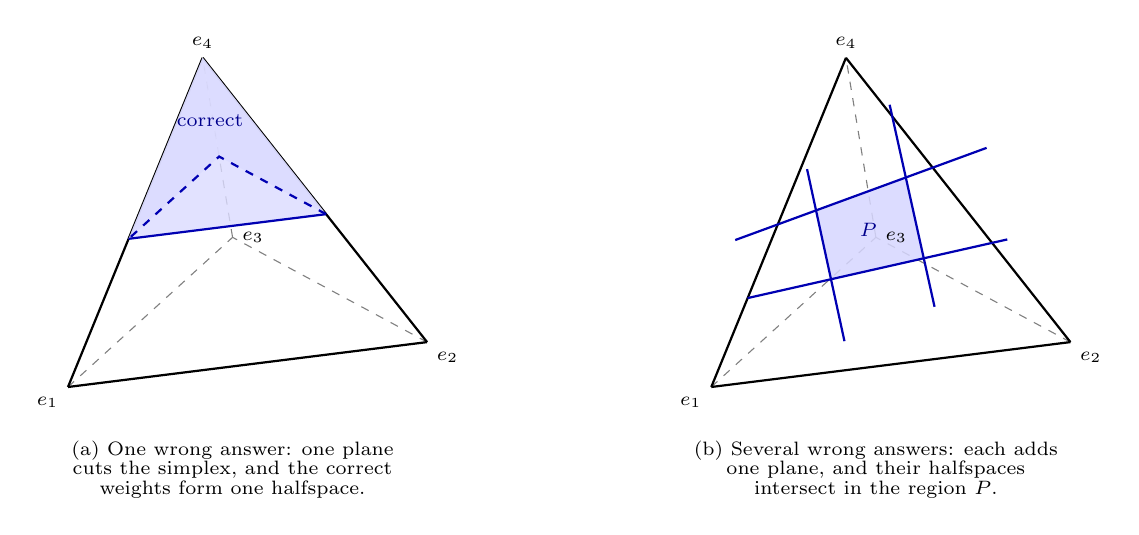
\begin{tikzpicture}[scale=1.9,every node/.style={font=\scriptsize}]
  \begin{scope}
    \coordinate (A) at (0,0);
    \coordinate (B) at (2.4,0.3);
    \coordinate (C) at (1.1,1.0);
    \coordinate (D) at (0.9,2.2);
    \draw[gray,dashed] (A)--(C) (B)--(C) (C)--(D);
    \draw[thick] (A)--(B) (A)--(D) (B)--(D);
    \coordinate (P1) at (0.405,0.99);
    \coordinate (P2) at (1.725,1.155);
    \coordinate (P3) at (1.01,1.54);
    \fill[blue!14,opacity=0.8] (P1)--(P2)--(D)--cycle;
    \fill[blue!14,opacity=0.8] (P1)--(P3)--(D)--cycle;
    \fill[blue!14,opacity=0.8] (P2)--(P3)--(D)--cycle;
    \draw[blue!70!black,thick] (P1)--(P2);
    \draw[blue!70!black,thick,dashed] (P2)--(P3)--(P1);
    \node[blue!55!black] at (0.95,1.78) {correct};
    \node[below left] at (A) {$e_1$};
    \node[below right] at (B) {$e_2$};
    \node[right] at (C) {$e_3$};
    \node[above] at (D) {$e_4$};
    \node[align=center] at (1.1,-0.55)
      {(a) One wrong answer: one plane\\[-1pt]cuts the simplex, and the correct\\[-1pt]weights form one halfspace.};
  \end{scope}
  \begin{scope}[xshift=4.3cm]
    \coordinate (A) at (0,0);
    \coordinate (B) at (2.4,0.3);
    \coordinate (C) at (1.1,1.0);
    \coordinate (D) at (0.9,2.2);
    \draw[gray,dashed] (A)--(C) (B)--(C) (C)--(D);
    \draw[thick] (A)--(B) (A)--(D) (B)--(D);
    \coordinate (Q1) at (0.80,0.72);
    \coordinate (Q2) at (1.42,0.86);
    \coordinate (Q3) at (1.30,1.40);
    \coordinate (Q4) at (0.70,1.18);
    \fill[blue!16,opacity=0.85] (Q1)--(Q2)--(Q3)--(Q4)--cycle;
    \draw[blue!70!black,thick] ($(Q1)!-0.9!(Q2)$)--($(Q2)!-0.9!(Q1)$);
    \draw[blue!70!black,thick] ($(Q2)!-0.6!(Q3)$)--($(Q3)!-0.9!(Q2)$);
    \draw[blue!70!black,thick] ($(Q3)!-0.9!(Q4)$)--($(Q4)!-0.9!(Q3)$);
    \draw[blue!70!black,thick] ($(Q4)!-0.6!(Q1)$)--($(Q1)!-0.9!(Q4)$);
    \node[blue!55!black] at (1.05,1.05) {$P$};
    \node[below left] at (A) {$e_1$};
    \node[below right] at (B) {$e_2$};
    \node[right] at (C) {$e_3$};
    \node[above] at (D) {$e_4$};
    \node[align=center] at (1.1,-0.55)
      {(b) Several wrong answers: each adds\\[-1pt]one plane, and their halfspaces\\[-1pt]intersect in the region $P$.};
  \end{scope}
\end{tikzpicture}
\caption{Correct-weight geometry for one question with \(K=4\).  The weight
simplex is a tetrahedron whose vertices are pure model choices.  Each contender
creates a decision hyperplane.  With one contender, correctness selects one
side of one plane; with several contenders, all inequalities must hold, giving
the relative interior of a polytope.}
\label{fig:weight-geometry}
\end{figure}

\subsection{Buffered empirical risk minimization}
\label{sec:method-buffer}

Raw empirical risk minimization can reward a weight vector for exploiting
finite-\(N\) sign errors near zero.  We instead require the empirical gold
score to clear a positive buffer.  For \(\varepsilon\ge0\), define
\begin{equation}
\widehat R_\varepsilon(w)
=
\frac1Q\sum_{j=1}^Q
\mathbf 1\{\widehat M_{q_j}(w)\le\varepsilon\},
\qquad
\widehat w_\varepsilon\in
\arg\min_{w\in\Delta_K}\widehat R_\varepsilon(w).
\label{eq:buffered-erm}
\end{equation}
The theory chooses
\(\varepsilon=\varepsilon_N(\delta)
=\sqrt{2\log(8KAQ/\delta)/N}\), the uniform training-sample scale of the
finite-generation error.  The constant is not essential; the statistical
role is.  A problem is counted as empirically solved only when the observed
gold score beats every observed contender by more than the uncertainty
radius.

\begin{algorithm}[t]
\caption{Margin-buffered weighted voting}
\label{alg:buffered}
\begin{algorithmic}[1]
\STATE \textbf{Input:} labeled problems \(q_{1:Q}\), models \(1{:}K\),
generation count \(N\), confidence \(\delta\)
\FOR{each training problem \(q_j\) and model \(i\)}
  \STATE draw \(N\) answers and compute the frequencies in
  Eq.~(\ref{eq:phat})
\ENDFOR
\STATE set
\(\varepsilon_N\leftarrow\sqrt{2\log(8KAQ/\delta)/N}\)
\STATE solve Eq.~(\ref{eq:buffered-erm}) for
\(\widehat w_{\varepsilon_N}\)
\STATE \textbf{return} the learned weights \(\widehat w_{\varepsilon_N}\)
\STATE \textbf{Deploy:} estimate fresh frequencies
\(\widehat p_i(\cdot\mid q)\)
\STATE \textbf{predict}
\(\widehat f_N(q)=\arg\max_a\sum_i\widehat w_{\varepsilon_N,i}
\widehat p_i(a\mid q)\)
\end{algorithmic}
\end{algorithm}

The main theorem isolates the effect of finite generations during weight
fitting: it controls the clean population risk
\(R(\widehat w_{\varepsilon_N})\), whose predictor uses the population scores
\(s_q(a;\widehat w_{\varepsilon_N})\).  The practical
\(\widehat f_N\) above incurs an additional prediction-time perturbation from
fresh generations.  Appendix~\ref{app:legacy-support} gives a sign-reliability
bound for any fixed weight; extending it uniformly to the data-dependent
\(\widehat w_{\varepsilon_N}\) requires boundary control beyond the one-sided
comparator condition used by Theorem~\ref{thm:buffered-main}.

\subsection{Exact optimization as a MILP}
\label{sec:method-milp}

The buffered objective is discontinuous but admits a direct mixed-integer
linear implementation.  Introduce \(z_j\in\{0,1\}\), where \(z_j=1\) claims
that problem \(j\) clears the buffer.  A solver uses a small strictness
tolerance \(\tau>0\) and any
\(B_{\rm M}\ge 1+\varepsilon_N+\tau\).  It solves
\begin{equation}
\max_{w\in\Delta_K,\,z\in\{0,1\}^Q}\sum_{j=1}^Qz_j
\quad\text{subject to}\quad
\langle w,\widehat\Delta_{q_j,a}\rangle
\ge
\varepsilon_N+\tau-B_{\rm M}(1-z_j)
\quad
\forall j,\ a\ne a^\star(q_j).
\label{eq:buffered-milp}
\end{equation}
If \(z_j=1\), every wrong answer must trail the gold answer by at least
\(\varepsilon_N+\tau\); if \(z_j=0\), the big-\(M\) term releases the
constraints.  Thus this is the exact MILP for the \(\tau\)-tightened buffered
objective, and it approaches Eq.~(\ref{eq:buffered-erm}) as
\(\tau\downarrow0\).
The implementation in \texttt{src/tte/milp.py} exposes the threshold as
\texttt{strict\_margin}.  Setting it to \(\varepsilon_N+\tau\) implements the
\(\tau\)-tightened objective.  The proof of Theorem~\ref{thm:buffered-main}
then goes through with the comparator band
\(0<M_q(w^\star)\le2\varepsilon_N+\tau\), provided
\(2\varepsilon_N+\tau\le t_0\).  Existing scripts that use \(10^{-4}\) employ
only a numerical tie-breaking margin and should not be described as evaluations
of the calibrated buffered estimator.

\section{Theoretical Analysis}
\label{sec:theory}

Let \(w^\star\in\arg\min_{w\in\Delta_K}R(w)\).  Our default guarantee needs
only a one-sided condition at this fixed comparator.

\begin{assumption}[Comparator margin condition]
\label{ass:comp-margin}
There are \(C_m>0\), \(\beta>0\), and \(t_0>0\) such that
\[
\mathbb P_{q\sim\mathcal D}
\{0<M_q(w^\star)\le t\}
\le C_m t^\beta,
\qquad 0<t\le t_0.
\]
\end{assumption}

This condition controls only correctly solved problems that are close to a
tie.  It says nothing about negative margins and, importantly, imposes no
margin condition at the random estimator.

\subsection{Uniform control of finite-generation margins}
\label{sec:theory-concentration}

\begin{lemma}[Uniform training-sample margin accuracy]
\label{lem:margin-accuracy}
For \(\delta\in(0,1)\), set
\(\varepsilon_N(\delta)=\sqrt{2\log(8KAQ/\delta)/N}\).  With probability at
least \(1-\delta/2\) over the generations, conditional on the sampled questions,
\[
\sup_{j\le Q}\sup_{w\in\Delta_K}
|\widehat M_{q_j}(w)-M_{q_j}(w)|
\le\varepsilon_N(\delta).
\]
\end{lemma}

\begin{proof}
Hoeffding's inequality and a union bound over at most \(KAQ\) answer
frequencies give
\[
\max_{j,i,a}
|\widehat p_i(a\mid q_j)-p_i(a\mid q_j)|
\le\frac{\varepsilon_N}{2}
\]
with probability at least \(1-\delta/2\).  Every coordinate of an answer-gap
vector then has error at most \(\varepsilon_N\).  Since
\(\|w\|_1=1\), each weighted gap has the same bound; stability of the minimum
over wrong answers preserves it.
\end{proof}

On this event, for every training question and every \(w\),
\begin{equation}
\mathbf 1\{M_{q_j}(w)\le0\}
\le
\mathbf 1\{\widehat M_{q_j}(w)\le\varepsilon_N\}
\le
\mathbf 1\{M_{q_j}(w)\le2\varepsilon_N\}.
\label{eq:indicator-sandwich}
\end{equation}
This uniform sandwich is the reason for introducing the buffer.

For \(t\ge0\), define
\(\mathcal F_t=\{q\mapsto\mathbf 1\{M_q(w)\le t\}:w\in\Delta_K\}\).
On \(Q\) fixed questions, at most \(Q(A-1)\) affine hyperplanes partition the
\((K-1)\)-dimensional simplex.  Thus
\[
\Pi_{\mathcal F_t}(Q)
\le
\sum_{r=0}^{K-1}\binom{Q(A-1)}r,
\]
and standard VC symmetrization yields, simultaneously for
\(t\in\{0,2\varepsilon_N\}\),
\begin{equation}
\sup_{w\in\Delta_K}
\left|
\frac1Q\sum_{j=1}^Q\mathbf 1\{M_{q_j}(w)\le t\}
-
\mathbb P\{M_q(w)\le t\}
\right|
\le
\mathfrak v_Q(\delta),
\label{eq:vq-event}
\end{equation}
where
\[
\mathfrak v_Q(\delta)
=
C\sqrt{
\frac{(K-1)\log(eAQ)+\log(1/\delta)}{Q}
}
\]
for a universal constant \(C\).

\subsection{The robust two-sample-size guarantee}
\label{sec:theory-main}

\begin{theorem}[Buffered ERM]
\label{thm:buffered-main}
Suppose Assumption~\ref{ass:comp-margin} holds and
\(2\varepsilon_N(\delta)\le t_0\).  Let
\(\widehat w_\varepsilon\) minimize
\(\widehat R_{\varepsilon_N}\) in Eq.~(\ref{eq:buffered-erm}).  With
probability at least \(1-\delta\) over both the \(Q\) questions and all
generations,
\begin{equation}
R(\widehat w_\varepsilon)-R(w^\star)
\le
2\mathfrak v_Q(\delta)
+
C_m(2\varepsilon_N(\delta))^\beta.
\label{eq:buffered-main-bound}
\end{equation}
Consequently,
\begin{equation}
R(\widehat w_\varepsilon)-R(w^\star)
\lesssim
\sqrt{\frac{(K-1)\log(eAQ)+\log(1/\delta)}{Q}}
+
C_m
\left(\frac{\log(KAQ/\delta)}{N}\right)^{\beta/2}.
\label{eq:buffered-rate}
\end{equation}
\end{theorem}

\begin{proof}
Write
\(\widetilde R_t(w)=Q^{-1}\sum_j\mathbf 1\{M_{q_j}(w)\le t\}\) and
\(R_t(w)=\mathbb P\{M_q(w)\le t\}\).  On the intersection of the events in
Lemma~\ref{lem:margin-accuracy} and Eq.~(\ref{eq:vq-event}),
\[
\begin{aligned}
R(\widehat w_\varepsilon)
&\le \widetilde R_0(\widehat w_\varepsilon)+\mathfrak v_Q \\
&\le \widehat R_{\varepsilon_N}(\widehat w_\varepsilon)+\mathfrak v_Q \\
&\le \widehat R_{\varepsilon_N}(w^\star)+\mathfrak v_Q \\
&\le \widetilde R_{2\varepsilon_N}(w^\star)+\mathfrak v_Q \\
&\le R_{2\varepsilon_N}(w^\star)+2\mathfrak v_Q.
\end{aligned}
\]
The remaining difference is exactly the positive comparator band:
\[
R_{2\varepsilon_N}(w^\star)-R(w^\star)
=
\mathbb P\{0<M_q(w^\star)\le2\varepsilon_N\}
\le C_m(2\varepsilon_N)^\beta.
\]
The two events have joint probability at least \(1-\delta\); substitution of
their definitions gives Eq.~(\ref{eq:buffered-rate}).
\end{proof}

The theorem separates two sources of uncertainty in learning the weights.  The
\(Q\)-term is ordinary generalization across questions.  The \(N\)-term is the
mass of comparator-correct training questions whose margins cannot be
distinguished from a tie at resolution \(N^{-1/2}\).  The latter can decay
faster than \(N^{-1/2}\) because the target is a thresholded correctness
decision rather than smooth parameter estimation.

\subsection{Why a margin condition does not imply a fast
\texorpdfstring{\(Q\)}{Q}-rate}
\label{sec:theory-obstruction}

The margin condition controls how much probability lies near a decision
boundary.  It does not say whether two well-separated regions of the weight
simplex have nearly identical risks.

\begin{proposition}[Hard margin with root-\(Q\) distinguishability]
\label{prop:counterexample}
There is a family with two models, two answers, \(N=\infty\), and a hard margin
at every optimum for which no learner can uniformly guarantee excess risk
\(o(Q^{-1/2})\) from \(Q\) labeled questions.
\end{proposition}

\begin{proof}
Write \(w=(t,1-t)\).  On type \(+\) questions, model 1 is always correct and
model 2 is always wrong, so \(M_q(w)=2t-1\).  On type \(-\) questions the
roles reverse and \(M_q(w)=1-2t\).  Consider distributions
\(\mathcal D_+\) and \(\mathcal D_-\) assigning type \(+\) probability
\(1/2+\eta/2\) and \(1/2-\eta/2\), respectively.  The optimal side of
\(t=1/2\) reverses between the two distributions; choosing the wrong side
costs excess risk \(\eta\).  At a pure optimal weight, every margin has
magnitude one, so there is no near-boundary mass.

Learning the correct side from \(Q\) questions is nevertheless testing two
coins with biases \(1/2\pm\eta/2\).  For
\(\eta=c/\sqrt Q\) with a sufficiently small constant \(c\), their
\(Q\)-sample laws have total variation bounded away from one.  Le Cam's
two-point argument therefore forces a constant probability of choosing the
wrong side under one of the distributions, and hence excess risk of order
\(Q^{-1/2}\).
\end{proof}

The obstruction is global identifiability, not boundary noise.  We therefore
state faster \(Q\)-rates only after adding a condition that risk grows when the
weights leave the optimum.

\subsection{Optional fast
\texorpdfstring{\(Q\)}{Q}-rates under identifiable geometry}
\label{sec:theory-fast}

\begin{assumption}[Absolute margin and risk growth]
\label{ass:growth}
There are \(C_m,\beta,t_0,c_g,\gamma,r_0,c_{\rm sep}>0\) such that
\begin{equation}
\mathbb P\{|M_q(w^\star)|\le t\}\le C_m t^\beta
\quad(0<t\le t_0),
\label{eq:absolute-margin}
\end{equation}
and
\begin{equation}
R(w)-R(w^\star)\ge
\begin{cases}
c_g\|w-w^\star\|_1^\gamma,
&\|w-w^\star\|_1\le r_0,\\
c_{\rm sep},
&\|w-w^\star\|_1>r_0.
\end{cases}
\label{eq:risk-growth}
\end{equation}
\end{assumption}

Let
\(D(w,w^\star)=\mathbb P\{\ell_q(w)\ne\ell_q(w^\star)\}\).

\begin{proposition}[Geometry implies a Bernstein condition]
\label{prop:geom-bernstein}
Under Assumption~\ref{ass:growth},
\begin{equation}
D(w,w^\star)
\le
B\{R(w)-R(w^\star)\}^{\alpha},
\qquad
\alpha=\min\{1,\beta/\gamma\},
\label{eq:bernstein-condition}
\end{equation}
for a finite constant \(B\).
\end{proposition}

\begin{proof}
Every contender gap is one-Lipschitz in \(\ell_1\), and taking a minimum
preserves that property.  If the losses at \(w\) and \(w^\star\) disagree,
then \(|M_q(w^\star)|\le\|w-w^\star\|_1\).  The absolute-margin condition
therefore gives
\(D(w,w^\star)\le C_m\|w-w^\star\|_1^\beta\) locally.  Inverting the local
risk-growth condition yields the exponent \(\beta/\gamma\); truncate it at
one because risks are bounded.  Outside the local ball, global separation and
\(D\le1\) complete the bound after enlarging the constant.  If
\(t_0<\|w-w^\star\|_1\le r_0\), the local growth condition itself gives
\(R(w)-R(w^\star)\ge c_gt_0^\gamma\), so this intermediate annulus is covered
by the same constant-enlargement argument.
\end{proof}

\begin{lemma}[Localized finite-growth bound]
\label{lem:localized-vc}
Let \(\mathcal L=\{\ell_q(w):w\in\Delta_K\}\) be a binary loss class with
minimizer \(w^\star\).  Suppose
\(\log\Pi_{\mathcal L}(n)\le V_n\) and \(V_{2Q}\le c_0V_Q\).  If
\[
\mathbb P\{\ell_q(w)\ne\ell_q(w^\star)\}
\le
B\{R(w)-R(w^\star)\}^{\alpha},
\qquad 0<\alpha\le1,
\]
and a data-dependent \(\widetilde w\) satisfies
\[
\frac1Q\sum_{j=1}^Q\ell_{q_j}(\widetilde w)
\le
\frac1Q\sum_{j=1}^Q\ell_{q_j}(w^\star)+a,
\]
then, with probability at least \(1-\delta\),
\begin{equation}
R(\widetilde w)-R(w^\star)
\le
C\left[
a+
\left(\frac{V_Q+\log(1/\delta)}{Q}\right)^{1/(2-\alpha)}
+\frac{V_Q+\log(1/\delta)}{Q}
\right],
\label{eq:localized-vc}
\end{equation}
where \(C\) depends only on \(B\), \(\alpha\), and \(c_0\).
\end{lemma}

\begin{proof}[Proof sketch]
For the excess loss \(g_w=\ell_q(w)-\ell_q(w^\star)\), the Bernstein premise
gives \(\mathbb E g_w^2\le B(\mathbb E g_w)^\alpha\).  Peeling the class into
shells \(r<\mathbb E g_w\le2r\), and applying Bernstein concentration with
the growth bound on each shell, gives deviation
\[
O\!\left(
\sqrt{\frac{r^\alpha\{V_Q+\log(1/\delta)\}}{Q}}
+\frac{V_Q+\log(1/\delta)}{Q}
\right).
\]
The fixed point in \(r\), together with the approximate-ERM slack \(a\),
yields Eq.~(\ref{eq:localized-vc}).  This is the standard relative
VC/localization argument \citep{massart2006risk,bartlett2005local,
koltchinskii2006local}; Appendix~\ref{app:fast-rate-proofs} gives the
specialization used here, including the \(2Q\)-sample growth step and the
data-dependent output.
\end{proof}

\begin{theorem}[Buffered ERM with an optional fast \(Q\)-rate]
\label{thm:fast}
Under Assumption~\ref{ass:growth}, let
\(\alpha=\min\{1,\beta/\gamma\}\).  For the same buffered estimator as in
Theorem~\ref{thm:buffered-main}, with probability at least \(1-\delta\),
\begin{equation}
R(\widehat w_\varepsilon)-R(w^\star)
\le
C
\left(
\frac{(K-1)\log(eAQ)+\log(1/\delta)}{Q}
\right)^{1/(2-\alpha)}
+
C'
\left(
\frac{\log(KAQ/\delta)}{N}
\right)^{\beta/2}.
\label{eq:fast-rate}
\end{equation}
The constants depend on the margin and growth parameters, not on
\(Q,N,K,\) or \(A\).
\end{theorem}

\begin{proof}[Proof sketch]
The indicator sandwich and optimality of the buffered estimator show that its
clean empirical risk exceeds that of \(w^\star\) by at most the empirical mass
of \(\{0<M_q(w^\star)\le2\varepsilon_N\}\).  Bernstein concentration for this
fixed band makes the slack
\(O(\varepsilon_N^\beta+\log(1/\delta)/Q)\).
Proposition~\ref{prop:geom-bernstein} supplies the Bernstein premise of
Lemma~\ref{lem:localized-vc}, with
\(V_Q=(K-1)\log(eAQ)\).  Applying that lemma to the preceding empirical slack
gives the localized \(Q\)-term; the band mass contributes the finite-\(N\)
term in Eq.~(\ref{eq:fast-rate}).  Appendix~\ref{app:fast-rate-proofs} tracks
the three confidence events and proves the full statement.
\end{proof}

The exponent is governed by two distinct geometric quantities.  \(\beta\)
measures the mass of questions that can change status near \(w^\star\);
\(\gamma\) measures how much the losses and gains fail to cancel when weights
move.  If crossings mostly hurt, then \(\gamma=\beta\), \(\alpha=1\), and the
\(Q\)-term is nearly \(Q^{-1}\).  If first-order losses and gains cancel, then
\(\gamma=\beta+1\), giving
\(\alpha=\beta/(\beta+1)\).  The latter exponent is a special geometry, not a
consequence of the margin condition by itself.

\section{Empirical Status and Direct Validation}
\label{sec:experiments}

The current evidence has two roles: it shows that finite-generation
instability is visible in the existing pipeline, and it identifies the
experiment still needed to test the calibrated buffer.  We keep those roles
separate.  In particular, none of the results below is presented as a completed
evaluation of Theorem~\ref{thm:buffered-main}.

\subsection{What the tracked artifacts establish}
\label{sec:experiments-existing}

The repository contains tracked generation files for AIME 2024, AIME 2025,
GPQA-Diamond, and MATH-500 \citep{rein2023gpqaag,hendrycks2021measuringmp}.
The reproducible analysis in
\texttt{zhi\_code/src/pacbayes\_boinf.py} compares the original weight-fitting
MILP with a bootstrap-stability plus max-margin variant.  Averaged over the four
benchmarks, the absolute train--test gap changes from \(0.0831\) to \(0.0717\),
or \(13.67\%\) relative closure.  Across five stored cross-benchmark
directions, the mean closure is \(26.00\%\), although the individual directions
are heterogeneous and one is negative.  The per-benchmark values, figures, and
artifact paths are reported in Appendix~\ref{app:legacy-real}; every stored
in-domain, transfer, model-count, and PAC--Bayes value is transcribed in
Appendix~\ref{app:legacy-full-data}.

These diagnostics establish that the code path is executable and that
regularizing a weight fit can change finite-sample generalization.  They do not
isolate the theorem's mechanism: the implemented variant combines bootstrap
stability with a numerical margin, whereas buffered ERM uses the explicit
uncertainty radius \(\varepsilon_N(\delta)\).  The retained PAC--Bayes values
are likewise diagnostics, not certificates for the deterministic buffered
predictor.

The earlier draft also reported a small synthetic mechanism check.  Its four
rows show the mass of the \(N^{-1/2}\) boundary band decreasing with \(N\),
while sign flips concentrate inside that band; a second column tracks the
selection bias from optimizing noisy empirical accuracy.  Because the original
per-replicate files are unavailable, Appendix~\ref{app:legacy-synthetic}
labels these values as legacy reports rather than a fresh rerun.

\subsection{The direct buffered-ERM experiment}
\label{sec:experiments-required}

A direct test should hold the model set and answer extractor fixed, repeatedly
split benchmark questions into training and test sets, and independently
subsample both axes: \(Q\) labeled training questions and \(N\) generations per
model and question.  On every split, it should compare uniform voting, raw ERM
with zero buffer, buffered ERM with
\(\varepsilon_N(\delta)=\sqrt{2\log(8KAQ/\delta)/N}\), and the existing
stability-plus-margin baseline.  The multiplicative constant in the buffer may
be selected on a validation split, but the test split must not influence it.

The primary outcomes are clean held-out error under high-generation
frequencies, end-to-end finite-generation held-out error, excess error relative
to a high-generation oracle fit, and the train--test gap.  Reporting the two
held-out errors separately prevents prediction-time sampling noise from being
mistaken for weight-estimation error.  Mechanism checks should also report the
empirical mass of the positive comparator band
\(0<M_q(w^\star)\le2\varepsilon_N\), margin-sign flips inside and outside that
band, and sensitivity to \(Q\), \(N\), \(K\), and the confidence level.  Repeated
splits or a paired bootstrap over questions should provide uncertainty
intervals.  This design distinguishes the \(Q\)-generalization term from the
\(N\)-resolution term instead of inferring both from one aggregate accuracy
curve.

\subsection{Implementation boundary}
\label{sec:experiments-implementation}

The existing solver in \texttt{src/tte/milp.py} already exposes the relevant
constraint through \texttt{strict\_margin}.  Passing
\(\varepsilon_N(\delta)\) implements Eq.~(\ref{eq:buffered-milp}); scripts that
pass \(10^{-4}\) use only a numerical tie-breaking tolerance.  Promoting the
planned experiment to a completed result therefore requires saved split
indices, sampled-generation indices, fitted weights, per-split metrics, and
the aggregate table or figure.  Until those artifacts exist, the theoretical
guarantee and the legacy diagnostics remain intentionally distinct.

The current matrix builder also forms each answer set from the union of answers
observed in the same finite generations.  A theorem-aligned run must instead
fix the answer normalization and candidate support before fitting, or define a
residual category whose treatment preserves the strongest-contender rule.
Otherwise an unobserved wrong answer can disappear from the empirical
\(\arg\max\), and the fixed-\(A\) concentration argument does not directly
describe the implemented decision rule.

\section{Limitations}
\label{sec:limitations}

The analysis assumes that candidate answers can be mapped to a finite set and
that generations are conditionally independent given a question and model.
Correlated decoding traces or unstable answer extraction would require a
different concentration radius.  The uniform radius is also conservative: it
pays a logarithmic factor for all observed model--answer--question
coordinates, even when many answers are rare or impossible.  Data-dependent
or variance-sensitive buffers may be substantially smaller.

The main guarantee targets the clean population risk of weights fitted from
finite-generation training margins.  A deployment that estimates answer
frequencies from fresh finite rollouts has a second perturbation.  The retained
fixed-weight sign bound describes that effect, but controlling it uniformly at
the random fitted weight would need an additional margin condition or a
selective prediction rule.

The optional fast \(Q\)-rate uses identifiable risk growth and global
separation.  These assumptions are intentionally stronger than a margin
condition and should be checked rather than treated as generic properties of
LLM benchmarks.  Finally, the tracked real-data analysis predates the
calibrated buffered estimator.  It supports the finite-sample motivation but
does not replace the direct \(Q\)-by-\(N\) evaluation specified in
Section~\ref{sec:experiments-required}.

\section{Conclusion}
\label{sec:conclusion}

Finite-generation ensemble weighting is governed by two sampling operations
that should not be collapsed into one.  Questions determine how well the
weight vector generalizes; generations determine whether a question's
gold-versus-contender margin can be resolved.  Buffering at the latter
uncertainty scale yields a clean comparison with the best fixed population
weight and a robust \(Q^{-1/2}+N^{-\beta/2}\) guarantee up to logarithmic
factors.  The hard-margin counterexample also draws a useful boundary: local
separation from zero is enough to control finite-generation errors, but not
enough to identify the best region of the weight simplex quickly.  Faster
learning across questions requires additional risk geometry.

This theorem hierarchy leaves a concrete empirical next step.  The existing
MILP already exposes the required margin threshold; a direct benchmark study
must now vary \(Q\) and \(N\), compare buffered and unbuffered fits, and retain
the split-level artifacts needed to distinguish the two terms.  Until then,
the theorem, the obstruction, and the legacy diagnostics make separate,
auditable claims.


\bibliography{buffered_erm_iclr2026}
\bibliographystyle{iclr2026_conference}

\clearpage
\appendix
\section{Legacy Results, Diagnostics, and Provenance}
\label{app:legacy}

This appendix records the material retained from the earlier draft.  The
current buffered analysis is authoritative: an older statement is carried
forward only when it is unchanged, follows under the assumptions used here, or
is explicitly marked as a result for a different observation model.
Table~\ref{tab:legacy-theory-map} makes that relationship explicit.

\begin{table}[t]
\centering
\small
\begin{tabular}{p{0.24\linewidth}p{0.31\linewidth}p{0.36\linewidth}}
\toprule
Earlier result & Status in this paper & Reason \\
\midrule
Correct-region polytope and MILP &
Retained in Section~\ref{sec:method-margin} and
Eq.~(\ref{eq:buffered-milp}) &
The geometry is unchanged; the MILP threshold is shifted by the calibrated
buffer and its numerical strictness tolerance is now explicit. \\
Uniform convergence over questions &
Retained as the slow-\(Q\) component of Theorem~\ref{thm:buffered-main} &
The hyperplane-arrangement argument gives complexity
\((K-1)\log(eAQ)\), without requiring a margin condition. \\
Accelerated \(Q\)-rate &
Replaced by Theorem~\ref{thm:fast} &
A margin condition alone is insufficient.  Fast learning additionally needs
absolute boundary control and identifiable risk growth. \\
Finite-generation \(N\)-term &
Retained and strengthened by buffering &
The buffer pays boundary mass only at the fixed comparator rather than
requiring a uniform margin condition at a random learned weight. \\
Joint \((N,Q)\) rate &
Replaced by Theorem~\ref{thm:buffered-main}, with an optional fast version in
Theorem~\ref{thm:fast} &
The robust default is \(Q^{-1/2}+N^{-\beta/2}\); a faster \(Q\)-term is
conditional on geometric identifiability. \\
Rollout minimax lower bound &
Retained below as a complementary observation-model result &
It concerns prediction from sampled answers with the gold answer hidden, not
the supervised weight-learning experiment of the main theorem. \\
Compute-allocation corollaries &
Not asserted as results of the buffered-only paper &
They depend on a chosen cost model and rate constants.  The old formulas
remain preserved in the untouched source draft, but are not needed for the
estimator or its guarantee. \\
\bottomrule
\end{tabular}
\caption{Disposition of the principal results from the earlier draft.  No
unsupported fast-\(Q\) claim is silently inherited.}
\label{tab:legacy-theory-map}
\end{table}

\subsection{Supporting finite-generation facts}
\label{app:legacy-support}

The first fact explains why taking the hardest wrong answer changes constants
but not the concentration scale.

\begin{lemma}[Stability of the minimum]
\label{lem:legacy-min-stability}
For finite vectors \(x=(x_a)_{a\in I}\) and \(y=(y_a)_{a\in I}\),
\[
\left|\min_{a\in I}x_a-\min_{a\in I}y_a\right|
\le \max_{a\in I}|x_a-y_a|.
\]
Consequently, for every problem \(q\) and \(w\in\Delta_K\),
\[
|\widehat M_q(w)-M_q(w)|
\le
\max_{a\ne a^\star(q)}
\left|\left\langle
w,\widehat\Delta_{q,a}-\Delta_{q,a}
\right\rangle\right|.
\]
\end{lemma}

\begin{proof}
Let \(a_x\) and \(a_y\) minimize \(x\) and \(y\), respectively.  Then
\(\min x-\min y=x_{a_x}-y_{a_y}\le x_{a_y}-y_{a_y}\le
\max_a|x_a-y_a|\).  Interchanging \(x\) and \(y\) gives the reverse
inequality.  The margin statement follows by substitution.
\end{proof}

\begin{lemma}[Fixed-weight sign reliability]
\label{lem:legacy-sign}
Assume independent generations across models and draws.  For fixed \(q,w\), let
\(m=|M_q(w)|>0\).  There is a universal \(c>0\) such that
\[
\mathbb P_{\rm gen}\!\left(
\mathbf 1\{\widehat M_q(w)\le0\}\ne
\mathbf 1\{M_q(w)\le0\}\mid q
\right)
\le
2(A-1)\exp\!\left(
-\frac{cNm^2}{\|w\|_2^2}
\right).
\]
In particular, the right side is at most
\(2(A-1)e^{-cNm^2}\) for \(w\in\Delta_K\).
\end{lemma}

\begin{proof}
For a fixed wrong answer \(a\), the empirical score-gap error is a weighted
sum of \(KN\) independent, centered, bounded variables.  Hoeffding's lemma
makes it sub-Gaussian with variance proxy \(C\|w\|_2^2/N\).  A sign change of
the minimum requires at least one contender gap to move by \(m\); apply the
sub-Gaussian tail bound and union bound over at most \(A-1\) contenders.
\end{proof}

The next counterexample is about the raw plug-in risk, not buffered ERM.  It
shows why a punctured condition that ignores mass exactly at zero cannot by
itself guarantee convergence of raw empirical signs.

\begin{proposition}[Zero-margin atom for raw plug-in risk]
\label{prop:legacy-zero-atom}
There is a one-model, two-answer instance satisfying
\(\mathbb P(0<|M_q(w^\star)|\le t)=0\) for every \(t>0\), while for every odd
\(N\),
\[
|R_N(w^\star)-R(w^\star)|=\frac12.
\]
\end{proposition}

\begin{proof}
Let the gold and wrong answers each have probability \(1/2\).  Then
\(M_q(w^\star)=0\), and ties count as errors, so \(R(w^\star)=1\).  If
\(Z\sim{\rm Binomial}(N,1/2)\), the empirical margin for odd \(N\) is
\((2Z-N)/N\), which is negative with probability \(1/2\).  Hence
\(R_N(w^\star)=1/2\).  Theorem~\ref{thm:buffered-main} does not make this
mistake: its one-sided comparator condition charges only the additional
positive-margin band created by the buffer.
\end{proof}

\begin{theorem}[Recovery of exact-output aggregation]
\label{thm:legacy-exact-limit}
Fix \(w\in\Delta_K\) and suppose
\(\mathbb P_q\{M_q(w)=0\}=0\).  If every empirical answer frequency is formed
from \(N\) independent generations, then
\[
\lim_{N\to\infty}
\mathbb P_{q,\rm gen}\{\widehat M_q^{(N)}(w)\le0\}
=
\mathbb P_q\{M_q(w)\le0\}.
\]
\end{theorem}

\begin{proof}
For fixed \(q\), the strong law and finiteness of the model and answer sets
give uniform coordinate convergence of empirical answer probabilities.
Lemma~\ref{lem:legacy-min-stability} then gives
\(\widehat M_q^{(N)}(w)\to M_q(w)\) almost surely.  The error indicator
converges away from zero, and the no-boundary-mass assumption plus dominated
convergence completes the proof.
\end{proof}

\begin{corollary}[Separated-margin finite-generation term]
\label{cor:legacy-separated}
If \(|M_q(w^\star)|\ge\gamma>0\) almost surely, then
\[
|R_N(w^\star)-R(w^\star)|
\le 2(A-1)e^{-cN\gamma^2}.
\]
\end{corollary}

\begin{proof}
Integrate Lemma~\ref{lem:legacy-sign} over \(q\) and use
\(\|w^\star\|_2\le1\).
\end{proof}

\subsection{A complementary rollout lower bound}
\label{app:legacy-lower-bound}

The supervised problem in the main text learns \(w\) from labeled questions.
The following retained theorem addresses a different prediction-time model:
the rule sees only \(N\) sampled binary answers and does not observe the gold
answer or an identifying problem feature.  Stating that distinction is
essential; the result is evidence that finite-generation ambiguity can be
information-theoretic, not a lower bound for every supervised protocol.

\begin{theorem}[Rollout-only minimax lower bound]
\label{thm:legacy-rollout-lower}
For \(\beta\ge0\) and \(C_m\ge1\), let
\(\mathfrak D_\beta(C_m)\) be the binary one-model distributions satisfying
\(\mathbb P(0<M_q\le t)\le C_m t^\beta\).  Under the rollout-only observation
model above, there is \(c_{\beta,C_m}>0\) such that
\[
\inf_{\psi_N}\sup_{\mathcal D\in\mathfrak D_\beta(C_m)}
\left\{
R_N^{\psi}(\mathcal D)-R_\infty^\star(\mathcal D)
\right\}
\ge c_{\beta,C_m}N^{-\beta/2}.
\]
\end{theorem}

\begin{proof}
Set \(\gamma_N=1/(8\sqrt N)\) and place mass
\(\alpha_N=c_\alpha\gamma_N^\beta\) on near-tie problems, where
\(c_\alpha=\min\{C_m/2,1/2\}\).  Conditional on the hidden gold bit, sampled
answers follow Bernoulli laws with means \((1+\gamma_N)/2\) and
\((1-\gamma_N)/2\).  Their \(N\)-fold KL divergence is bounded by a universal
constant, so Le Cam's two-point bound gives testing error at least \(3/8\).
The infinite-rollout oracle is correct, while every finite rule incurs at
least \((3/8)\alpha_N\), which is the displayed order.  The remaining mass can
be placed on deterministic easy problems, and the construction satisfies the
stated margin condition.
\end{proof}

\subsection{Legacy mechanism checks}
\label{app:legacy-synthetic}

Table~\ref{tab:legacy-synthetic} preserves the two small simulations reported
in the earlier note.  They are useful mechanism checks, but the original
per-replicate artifacts are unavailable; the numbers are therefore reported as
legacy values rather than a fresh rerun.  The first four columns show that
sign errors concentrate in the \(N^{-1/2}\) boundary band.  The last column
reports optimization bias at fixed \(Q=60\).

\begin{table}[t]
\centering
\small
\begin{tabular}{rcccc}
\toprule
\(N\) & band mass & in-band flip & out-of-band flip &
in-sample minus true accuracy \\
\midrule
20   & 0.465 & 0.189 & 0.004 & 0.054 \\
80   & 0.252 & 0.175 & 0.002 & 0.029 \\
320  & 0.119 & 0.198 & 0.001 & 0.018 \\
1280 & 0.060 & 0.192 & 0.000 & 0.013 \\
\bottomrule
\end{tabular}
\caption{Legacy synthetic mechanism checks.  Band mass is
\(\mathbb P(|M_q|\le N^{-1/2})\); flip columns condition on being inside or
outside that band.  The final column is the earlier winner-selection diagnostic
at fixed \(Q=60\).}
\label{tab:legacy-synthetic}
\end{table}

\subsection{Reproducible benchmark context}
\label{app:legacy-real}

We also retain a reproducible legacy analysis over tracked generation JSONL
files.  It compares the original MILP with a bootstrap-stability plus
max-margin variant; it does \emph{not} evaluate the statistically calibrated
buffer \(\varepsilon_N\) of Theorem~\ref{thm:buffered-main}.  Accordingly,
Table~\ref{tab:legacy-real} is context for the empirical motivation, not direct
validation of the new estimator.

\begin{table}[t]
\centering
\small
\begin{tabular}{lrrrr}
\toprule
Benchmark & \(Q\) & \(K\) & vanilla gap & stability+margin gap \\
\midrule
AIME 2024    & 30  & 11 & 0.0951 & 0.0946 \\
AIME 2025    & 30  & 11 & 0.1523 & 0.1279 \\
GPQA-Diamond & 198 & 6  & 0.0683 & 0.0494 \\
MATH-500     & 500 & 7  & 0.0167 & 0.0150 \\
\bottomrule
\end{tabular}
\caption{Absolute train--test gaps from the reproducible legacy JSONL
analysis.  Averaged over benchmarks, the gap falls from \(0.0831\) to
\(0.0717\), a \(13.67\%\) closure.}
\label{tab:legacy-real}
\end{table}

The same run reports \(26.00\%\) mean gap closure across the five stored
cross-benchmark directions.  These aggregate values are descriptive because
the benchmark sizes, model sets, and train fractions differ.

\begin{table}[t]
\centering
\small
\begin{tabular}{lrrr}
\toprule
Benchmark & \(Q\) & empirical risk & uniform-prior bound \\
\midrule
AIME 2024    & 30  & 0.000 & 2.216 \\
AIME 2025    & 30  & 0.200 & 2.277 \\
GPQA-Diamond & 198 & 0.250 & 0.541 \\
MATH-500     & 500 & 0.023 & 0.369 \\
\bottomrule
\end{tabular}
\caption{Retained PAC--Bayes diagnostic from the same run.  The AIME bounds
are vacuous; the table is not used in any theorem.}
\label{tab:legacy-pacbayes}
\end{table}

\begin{figure}[t]
\centering
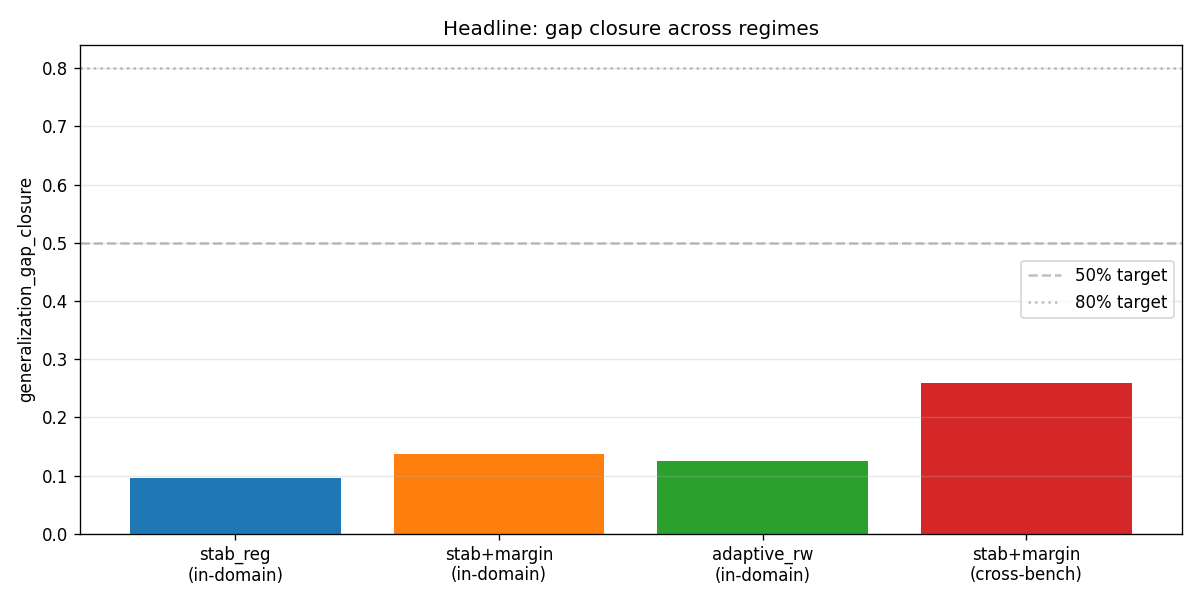
\includegraphics[width=0.49\linewidth]{buffered_figures/legacy_gap_closure.png}
\hfill
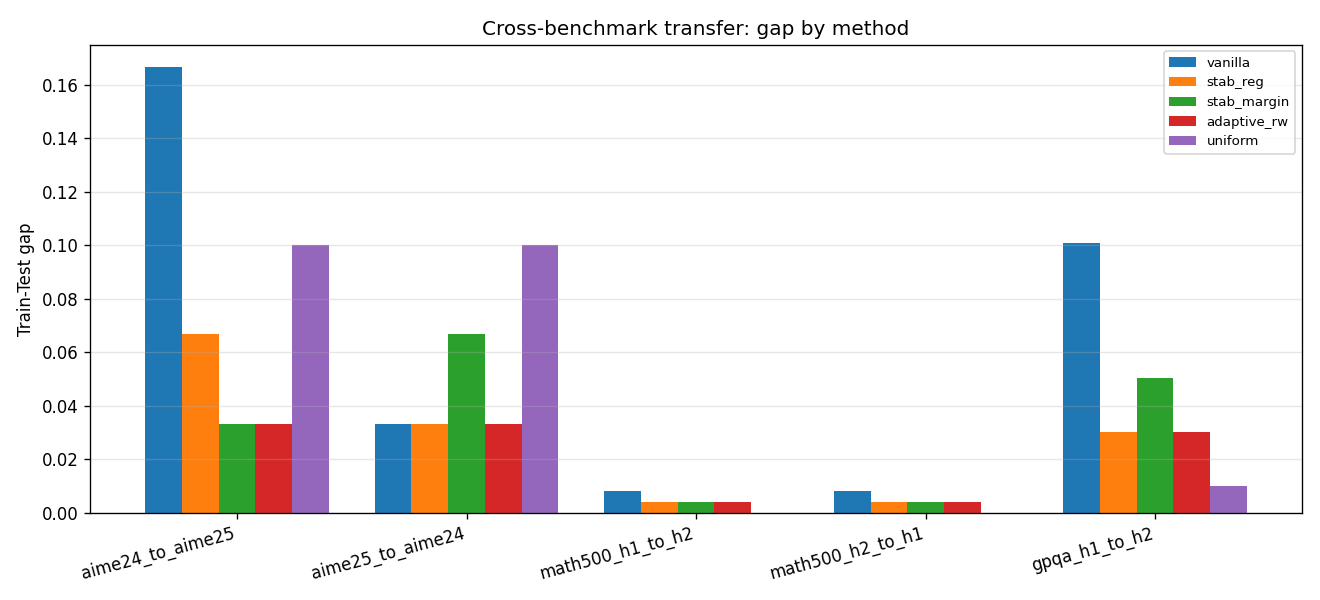
\includegraphics[width=0.49\linewidth]{buffered_figures/legacy_cross_benchmark.png}
\caption{Reproducible legacy diagnostics.  Left: in-domain gap closure.
Right: cross-benchmark train--test gaps.  Both figures are regenerated from
the tracked JSONL files by \texttt{zhi\_code/src/pacbayes\_boinf.py}.}
\label{fig:legacy-gap}
\end{figure}

\begin{figure}[t]
\centering
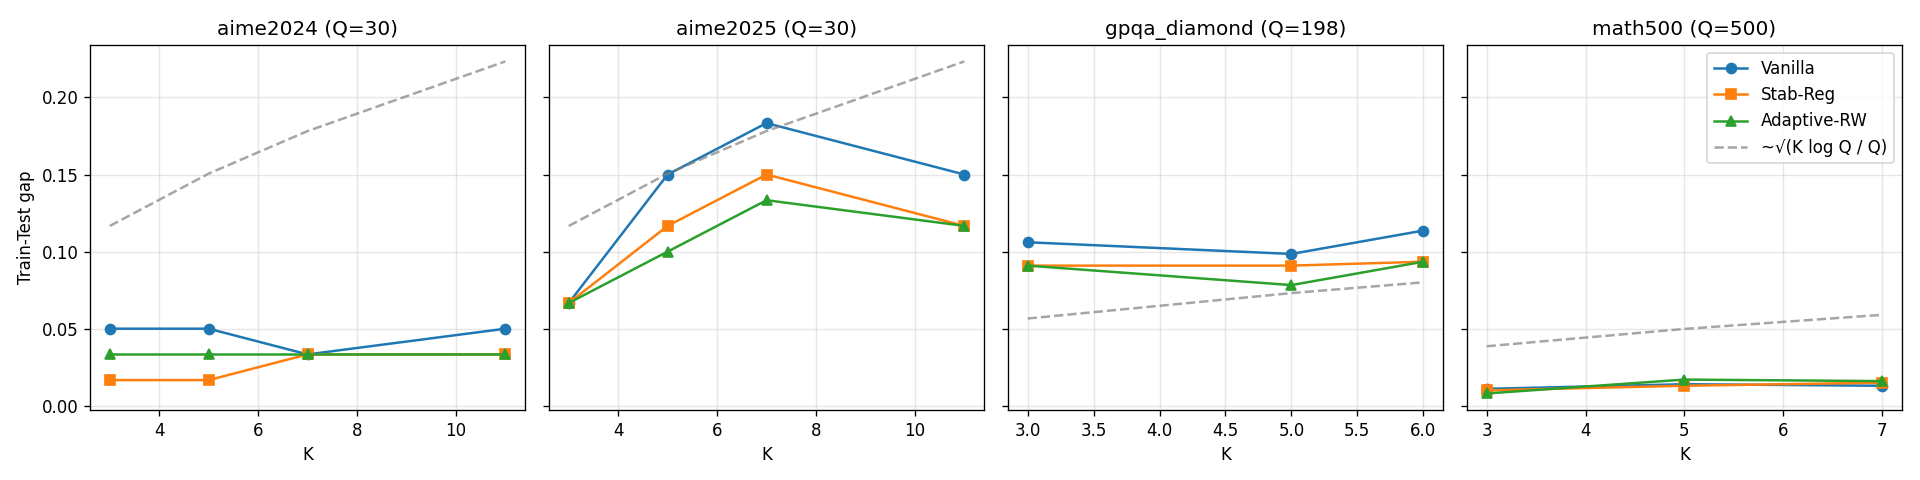
\includegraphics[width=0.49\linewidth]{buffered_figures/legacy_k_scaling.png}
\hfill
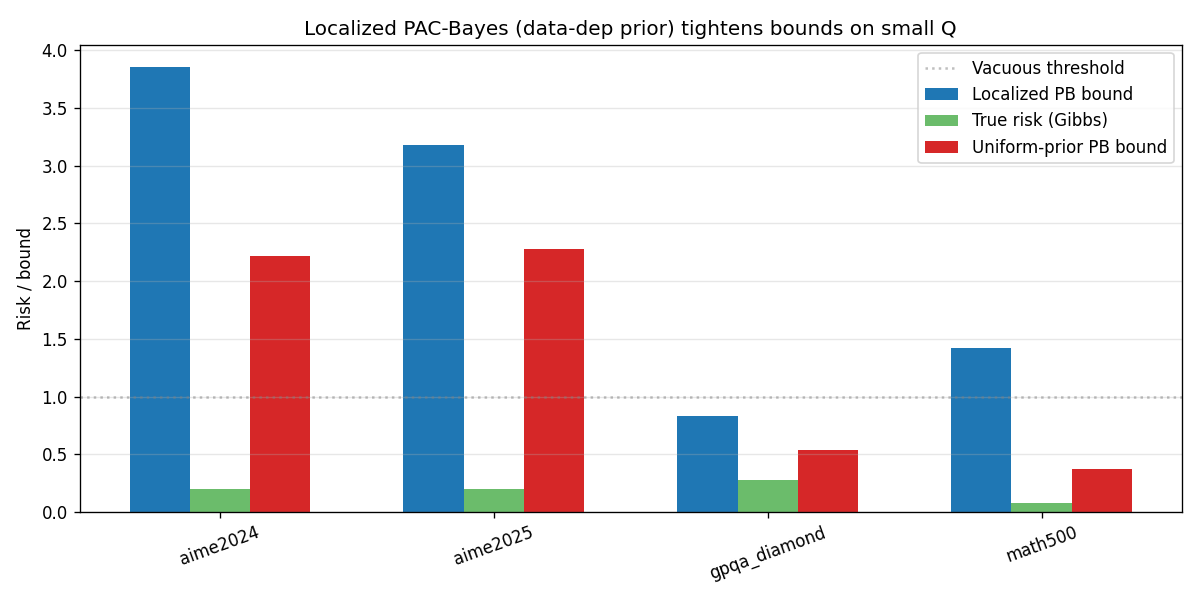
\includegraphics[width=0.49\linewidth]{buffered_figures/legacy_pac_bayes.png}
\caption{Additional retained diagnostics.  Left: dependence of measured gaps
on the number of ensemble members.  Right: localized and uniform-prior
PAC--Bayes values.  These are auxiliary diagnostics rather than evidence for
the buffered-ERM theorem.}
\label{fig:legacy-aux}
\end{figure}

\paragraph{Artifact record.}
The complete numerical object is
\path{zhi_code/src/working/experiment_data.json}; plots are in the same
directory.  The inputs are the tracked files under
\path{zhi_code/reference_data/jsonl}.  Appendix~\ref{app:legacy-full-data}
transcribes every field with completed numerical content in that object.  The
expanded synthetic tables in the earlier long appendix are omitted because no
matching saved artifacts were found.

\clearpage
\section{Detailed Proof of the Optional Fast Rate}
\label{app:fast-rate-proofs}

This appendix supplies the empirical-process details suppressed in
Section~\ref{sec:theory-fast}.  The argument is conditional on the stronger
absolute-margin and risk-growth assumptions; it is not needed for the default
bound in Theorem~\ref{thm:buffered-main}.

\subsection{Localized finite-growth lemma}

We prove Lemma~\ref{lem:localized-vc}.  Write \(P\) for expectation over a fresh
question, \(P_Q\) for the empirical mean over the \(Q\) training questions, and
\[
g_w(q)=\ell_q(w)-\ell_q(w^\star),
\qquad
r(w)=Pg_w=R(w)-R(w^\star).
\]
Because the losses are binary, \(g_w\in\{-1,0,1\}\) and
\[
Pg_w^2
=
\mathbb P\{\ell_q(w)\ne\ell_q(w^\star)\}
\le
B r(w)^\alpha.
\tag{A}
\label{eq:app-bernstein-second-moment}
\]

We use the standard relative VC deviation inequality for bounded excess losses
under a Bernstein condition \citep{massart2006risk,bartlett2005local,
koltchinskii2006local}.  For completeness, its specialization here is as
follows.  Peel the class into deterministic shells
\(\mathcal G_j=\{g_w:2^j\rho<r(w)\le2^{j+1}\rho\}\).  Ghost-sample
symmetrization reduces each shell to at most
\(\Pi_{\mathcal L}(2Q)\) restriction vectors.  Bernstein's inequality, (A), and
a union bound over those vectors and shells give, with probability at least
\(1-\delta\), simultaneously for all \(w\) with \(r(w)>\rho\),
\[
(P-P_Q)g_w
\le
c\left[
\sqrt{\frac{B r(w)^\alpha H_Q}{Q}}
+
\frac{H_Q}{Q}
\right],
\tag{B}
\label{eq:app-relative-vc}
\]
where \(H_Q=V_{2Q}+\log(1/\delta)+O(\log\log Q)\).
The ensemble arrangement bound holds at every sample size and satisfies
\(V_{2Q}\le c_0V_Q\).  Moreover,
\(V_Q\asymp(K-1)\log(eAQ)\) absorbs the shell-union
\(O(\log\log Q)\) term when \(K\ge2\).  The case \(K=1\) is trivial because the
simplex contains only one weight.  Thus \(H_Q\le
c_1\{V_Q+\log(1/\delta)\}\).  This is the usual finite-growth version of the
localized VC argument; the use of the \(2Q\)-sample growth function is what
makes (B) uniform over a data-dependent output.

Set \(h=\{V_Q+\log(1/\delta)\}/Q\) and
\(\rho=h^{1/(2-\alpha)}+h\).  If
\(r(\widetilde w)\le\rho\), the claimed result is immediate.  Otherwise, the
approximate-ERM premise gives \(P_Qg_{\widetilde w}\le a\), and (B) gives
\[
r(\widetilde w)
\le
a+c_2\sqrt B\,r(\widetilde w)^{\alpha/2}h^{1/2}+c_2h.
\]
Young's inequality with conjugate exponents \(2/\alpha\) and
\(2/(2-\alpha)\) yields
\[
c_2\sqrt B\,r^{\alpha/2}h^{1/2}
\le
\frac12r+c_3h^{1/(2-\alpha)},
\]
where \(c_3\) depends only on \(B\) and \(\alpha\).  Rearranging proves
\[
R(\widetilde w)-R(w^\star)
\le
C\left[
a+
\left(\frac{V_Q+\log(1/\delta)}{Q}\right)^{1/(2-\alpha)}
+
\frac{V_Q+\log(1/\delta)}{Q}
\right].
\]

\subsection{Buffered ERM is an approximate clean ERM}

We now complete Theorem~\ref{thm:fast}.  Let
\(\varepsilon_N=\sqrt{2\log(8KAQ/\delta)/N}\), and define the event
\[
\mathcal E_{\rm mar}
=
\left\{
\sup_{j\le Q}\sup_{w\in\Delta_K}
|\widehat M_{q_j}(w)-M_{q_j}(w)|
\le\varepsilon_N
\right\}.
\]
Lemma~\ref{lem:margin-accuracy} gives this event with the required conditional
high probability over generations.  On \(\mathcal E_{\rm mar}\), the indicator
sandwich and optimality of buffered ERM imply
\[
\begin{aligned}
P_Q\ell_{\widehat w_\varepsilon}
&\le
\widehat R_{\varepsilon_N}(\widehat w_\varepsilon)\\
&\le
\widehat R_{\varepsilon_N}(w^\star)\\
&\le
P_Q\mathbf 1\{M_q(w^\star)\le2\varepsilon_N\}\\
&=
P_Q\ell_{w^\star}
+
P_Q\mathbf 1\{0<M_q(w^\star)\le2\varepsilon_N\}.
\end{aligned}
\tag{C}
\label{eq:app-approx-erm-chain}
\]
This comparison uses distributional boundary control only at the fixed
comparator \(w^\star\), not at the random fitted weight.

Let \(B_N(q)=\mathbf 1\{0<M_q(w^\star)\le2\varepsilon_N\}\) and
\(b_N=PB_N\).  The absolute-margin condition and
\(2\varepsilon_N\le t_0\) give
\(b_N\le C_m(2\varepsilon_N)^\beta\).
Bernstein's inequality for the \(Q\) i.i.d.\ Bernoulli variables \(B_N(q_j)\)
gives, with probability at least \(1-\delta/4\),
\[
P_QB_N
\le
b_N+\sqrt{\frac{2b_N\log(4/\delta)}{Q}}
+
\frac{2\log(4/\delta)}{3Q}
\le
2b_N+\frac{2\log(4/\delta)}{Q}.
\tag{E}
\label{eq:app-band-concentration}
\]
The second inequality uses \(\sqrt{uv}\le(u+v)/2\).

On the intersection of the margin and band events, (C), the bound on \(b_N\),
and (E) show that
\(\widehat w_\varepsilon\) satisfies Lemma~\ref{lem:localized-vc} with the
deterministic slack
\[
a_N
=
2C_m(2\varepsilon_N)^\beta
+
\frac{2\log(4/\delta)}{Q}.
\]
Proposition~\ref{prop:geom-bernstein} supplies the lemma's Bernstein premise
with \(\alpha=\min\{1,\beta/\gamma\}\), and the hyperplane arrangement gives
\(V_Q\lesssim(K-1)\log(eAQ)\).  Applying the localized lemma at confidence
\(\delta/2\), and union-bounding its question-sample event with the margin and
band events, gives probability at least \(1-\delta\) and
\[
\begin{aligned}
R(\widehat w_\varepsilon)-R(w^\star)
\le C\Bigg[
&\left(
\frac{(K-1)\log(eAQ)+\log(1/\delta)}{Q}
\right)^{1/(2-\alpha)}\\
&+
\frac{(K-1)\log(eAQ)+\log(1/\delta)}{Q}
+
(2\varepsilon_N)^\beta
\Bigg].
\end{aligned}
\]
For normalized question complexity at most one, the linear term is no larger
than the localized power; when it exceeds one, the risk bound is trivial after
enlarging the constant.  Finally,
\[
(2\varepsilon_N)^\beta
\lesssim
\left(\frac{\log(KAQ/\delta)}{N}\right)^{\beta/2}.
\]
This proves Eq.~(\ref{eq:fast-rate}).  The conditional generation guarantee for
\(\mathcal E_{\rm mar}\) combines with the two question-sample events by the
tower property; no independence among the three events is required.

% Generated by scripts/export_buffered_legacy_tables.py.
\section{Complete Traceable Legacy Data}
\label{app:legacy-full-data}

This appendix transcribes every completed numerical object in \path{zhi_code/src/working/experiment_data.json}.  All results are legacy diagnostics: none fits the concentration-calibrated buffered estimator of Theorem~\ref{thm:buffered-main}.  The original split study stored aggregate means and population standard deviations over ten runs, but not the per-run observations.  We can therefore report marginal intervals for each mean, but cannot reconstruct paired tests between methods.

For a stored mean \(\bar x\), population standard deviation \(s_0\), and \(n=10\), the displayed interval is \(\bar x\mathbin{\pm}t_{0.975,9}s_0/\sqrt{n-1}\).  The archived script seeded each split with a process-dependent Python hash of the dataset name, so exact split indices are not recoverable from these summaries alone.

\subsection{In-domain train--test splits}

\begin{table*}[p]
\centering
\scriptsize
\setlength{\tabcolsep}{4pt}
\renewcommand{\arraystretch}{0.96}
\begin{tabular}{clcccc}
\toprule
Train fraction & Archived procedure & Train accuracy & Test accuracy & Absolute gap & \(95\%\) CI for mean gap \\
\midrule
0.3 & Raw ERM & \(0.933\mathbin{\pm}0.054\) & \(0.924\mathbin{\pm}0.044\) & \(0.086\mathbin{\pm}0.038\) & \([0.057,0.114]\) \\
0.3 & Uniform & \(0.933\mathbin{\pm}0.054\) & \(0.933\mathbin{\pm}0.023\) & \(0.076\mathbin{\pm}0.016\) & \([0.064,0.088]\) \\
0.3 & Best single & \(0.933\mathbin{\pm}0.054\) & \(0.886\mathbin{\pm}0.038\) & \(0.073\mathbin{\pm}0.062\) & \([0.026,0.120]\) \\
0.3 & Stability & \(0.933\mathbin{\pm}0.054\) & \(0.933\mathbin{\pm}0.023\) & \(0.076\mathbin{\pm}0.016\) & \([0.064,0.088]\) \\
0.3 & Stability \(+\) margin & \(0.933\mathbin{\pm}0.054\) & \(0.933\mathbin{\pm}0.023\) & \(0.076\mathbin{\pm}0.016\) & \([0.064,0.088]\) \\
0.3 & Adaptive reweighting & \(0.933\mathbin{\pm}0.054\) & \(0.933\mathbin{\pm}0.023\) & \(0.076\mathbin{\pm}0.016\) & \([0.064,0.088]\) \\
\midrule
0.5 & Raw ERM & \(0.913\mathbin{\pm}0.052\) & \(0.953\mathbin{\pm}0.052\) & \(0.093\mathbin{\pm}0.061\) & \([0.047,0.139]\) \\
0.5 & Uniform & \(0.913\mathbin{\pm}0.052\) & \(0.953\mathbin{\pm}0.052\) & \(0.093\mathbin{\pm}0.061\) & \([0.047,0.139]\) \\
0.5 & Best single & \(0.913\mathbin{\pm}0.052\) & \(0.893\mathbin{\pm}0.085\) & \(0.113\mathbin{\pm}0.073\) & \([0.058,0.169]\) \\
0.5 & Stability & \(0.913\mathbin{\pm}0.052\) & \(0.953\mathbin{\pm}0.052\) & \(0.093\mathbin{\pm}0.061\) & \([0.047,0.139]\) \\
0.5 & Stability \(+\) margin & \(0.913\mathbin{\pm}0.052\) & \(0.953\mathbin{\pm}0.052\) & \(0.093\mathbin{\pm}0.061\) & \([0.047,0.139]\) \\
0.5 & Adaptive reweighting & \(0.913\mathbin{\pm}0.052\) & \(0.953\mathbin{\pm}0.052\) & \(0.093\mathbin{\pm}0.061\) & \([0.047,0.139]\) \\
\midrule
0.7 & Raw ERM & \(0.933\mathbin{\pm}0.038\) & \(0.922\mathbin{\pm}0.087\) & \(0.106\mathbin{\pm}0.063\) & \([0.059,0.154]\) \\
0.7 & Uniform & \(0.933\mathbin{\pm}0.038\) & \(0.933\mathbin{\pm}0.089\) & \(0.114\mathbin{\pm}0.055\) & \([0.073,0.156]\) \\
0.7 & Best single & \(0.933\mathbin{\pm}0.038\) & \(0.878\mathbin{\pm}0.116\) & \(0.132\mathbin{\pm}0.092\) & \([0.062,0.201]\) \\
0.7 & Stability & \(0.933\mathbin{\pm}0.038\) & \(0.933\mathbin{\pm}0.089\) & \(0.114\mathbin{\pm}0.055\) & \([0.073,0.156]\) \\
0.7 & Stability \(+\) margin & \(0.933\mathbin{\pm}0.038\) & \(0.933\mathbin{\pm}0.089\) & \(0.114\mathbin{\pm}0.055\) & \([0.073,0.156]\) \\
0.7 & Adaptive reweighting & \(0.933\mathbin{\pm}0.038\) & \(0.933\mathbin{\pm}0.089\) & \(0.114\mathbin{\pm}0.055\) & \([0.073,0.156]\) \\
\bottomrule
\end{tabular}
\caption{Complete legacy AIME 2024 split results, with \(Q=30\), \(K=11\), and ten repeats.  Train/test counts are 9/21, 15/15, 21/9.  Entries are mean \(\mathbin{\pm}\) population standard deviation; the final column contains reconstructed marginal intervals.}
\label{tab:legacy-full-aime2024}
\end{table*}

\begin{table*}[p]
\centering
\scriptsize
\setlength{\tabcolsep}{4pt}
\renewcommand{\arraystretch}{0.96}
\begin{tabular}{clcccc}
\toprule
Train fraction & Archived procedure & Train accuracy & Test accuracy & Absolute gap & \(95\%\) CI for mean gap \\
\midrule
0.3 & Raw ERM & \(0.922\mathbin{\pm}0.112\) & \(0.862\mathbin{\pm}0.054\) & \(0.137\mathbin{\pm}0.090\) & \([0.069,0.204]\) \\
0.3 & Uniform & \(0.822\mathbin{\pm}0.142\) & \(0.838\mathbin{\pm}0.061\) & \(0.143\mathbin{\pm}0.145\) & \([0.033,0.253]\) \\
0.3 & Best single & \(0.922\mathbin{\pm}0.112\) & \(0.857\mathbin{\pm}0.064\) & \(0.160\mathbin{\pm}0.088\) & \([0.094,0.227]\) \\
0.3 & Stability & \(0.900\mathbin{\pm}0.144\) & \(0.876\mathbin{\pm}0.049\) & \(0.148\mathbin{\pm}0.109\) & \([0.065,0.230]\) \\
0.3 & Stability \(+\) margin & \(0.922\mathbin{\pm}0.112\) & \(0.890\mathbin{\pm}0.048\) & \(0.140\mathbin{\pm}0.083\) & \([0.077,0.203]\) \\
0.3 & Adaptive reweighting & \(0.922\mathbin{\pm}0.112\) & \(0.881\mathbin{\pm}0.044\) & \(0.137\mathbin{\pm}0.080\) & \([0.076,0.197]\) \\
\midrule
0.5 & Raw ERM & \(0.933\mathbin{\pm}0.067\) & \(0.813\mathbin{\pm}0.088\) & \(0.160\mathbin{\pm}0.104\) & \([0.081,0.239]\) \\
0.5 & Uniform & \(0.860\mathbin{\pm}0.092\) & \(0.807\mathbin{\pm}0.092\) & \(0.160\mathbin{\pm}0.104\) & \([0.081,0.239]\) \\
0.5 & Best single & \(0.933\mathbin{\pm}0.067\) & \(0.820\mathbin{\pm}0.095\) & \(0.153\mathbin{\pm}0.119\) & \([0.063,0.243]\) \\
0.5 & Stability & \(0.927\mathbin{\pm}0.081\) & \(0.847\mathbin{\pm}0.067\) & \(0.133\mathbin{\pm}0.099\) & \([0.059,0.208]\) \\
0.5 & Stability \(+\) margin & \(0.933\mathbin{\pm}0.067\) & \(0.860\mathbin{\pm}0.063\) & \(0.127\mathbin{\pm}0.076\) & \([0.070,0.184]\) \\
0.5 & Adaptive reweighting & \(0.933\mathbin{\pm}0.067\) & \(0.867\mathbin{\pm}0.067\) & \(0.133\mathbin{\pm}0.067\) & \([0.083,0.184]\) \\
\midrule
0.7 & Raw ERM & \(0.914\mathbin{\pm}0.036\) & \(0.811\mathbin{\pm}0.122\) & \(0.160\mathbin{\pm}0.090\) & \([0.092,0.228]\) \\
0.7 & Uniform & \(0.838\mathbin{\pm}0.049\) & \(0.822\mathbin{\pm}0.113\) & \(0.143\mathbin{\pm}0.078\) & \([0.084,0.201]\) \\
0.7 & Best single & \(0.914\mathbin{\pm}0.036\) & \(0.833\mathbin{\pm}0.102\) & \(0.138\mathbin{\pm}0.075\) & \([0.082,0.195]\) \\
0.7 & Stability & \(0.890\mathbin{\pm}0.052\) & \(0.833\mathbin{\pm}0.102\) & \(0.146\mathbin{\pm}0.072\) & \([0.091,0.201]\) \\
0.7 & Stability \(+\) margin & \(0.910\mathbin{\pm}0.040\) & \(0.878\mathbin{\pm}0.092\) & \(0.117\mathbin{\pm}0.068\) & \([0.066,0.169]\) \\
0.7 & Adaptive reweighting & \(0.905\mathbin{\pm}0.048\) & \(0.878\mathbin{\pm}0.092\) & \(0.122\mathbin{\pm}0.071\) & \([0.069,0.176]\) \\
\bottomrule
\end{tabular}
\caption{Complete legacy AIME 2025 split results, with \(Q=30\), \(K=11\), and ten repeats.  Train/test counts are 9/21, 15/15, 21/9.  Entries are mean \(\mathbin{\pm}\) population standard deviation; the final column contains reconstructed marginal intervals.}
\label{tab:legacy-full-aime2025}
\end{table*}

\begin{table*}[p]
\centering
\scriptsize
\setlength{\tabcolsep}{4pt}
\renewcommand{\arraystretch}{0.96}
\begin{tabular}{clcccc}
\toprule
Train fraction & Archived procedure & Train accuracy & Test accuracy & Absolute gap & \(95\%\) CI for mean gap \\
\midrule
0.3 & Raw ERM & \(0.805\mathbin{\pm}0.031\) & \(0.724\mathbin{\pm}0.025\) & \(0.081\mathbin{\pm}0.049\) & \([0.043,0.118]\) \\
0.3 & Uniform & \(0.732\mathbin{\pm}0.039\) & \(0.732\mathbin{\pm}0.017\) & \(0.048\mathbin{\pm}0.028\) & \([0.027,0.070]\) \\
0.3 & Best single & \(0.759\mathbin{\pm}0.041\) & \(0.717\mathbin{\pm}0.026\) & \(0.057\mathbin{\pm}0.053\) & \([0.017,0.097]\) \\
0.3 & Stability & \(0.754\mathbin{\pm}0.047\) & \(0.719\mathbin{\pm}0.017\) & \(0.053\mathbin{\pm}0.041\) & \([0.023,0.084]\) \\
0.3 & Stability \(+\) margin & \(0.758\mathbin{\pm}0.046\) & \(0.724\mathbin{\pm}0.019\) & \(0.060\mathbin{\pm}0.034\) & \([0.034,0.085]\) \\
0.3 & Adaptive reweighting & \(0.758\mathbin{\pm}0.046\) & \(0.729\mathbin{\pm}0.014\) & \(0.054\mathbin{\pm}0.033\) & \([0.028,0.079]\) \\
\midrule
0.5 & Raw ERM & \(0.783\mathbin{\pm}0.020\) & \(0.726\mathbin{\pm}0.030\) & \(0.063\mathbin{\pm}0.041\) & \([0.031,0.094]\) \\
0.5 & Uniform & \(0.728\mathbin{\pm}0.020\) & \(0.736\mathbin{\pm}0.020\) & \(0.034\mathbin{\pm}0.024\) & \([0.017,0.052]\) \\
0.5 & Best single & \(0.747\mathbin{\pm}0.025\) & \(0.717\mathbin{\pm}0.036\) & \(0.051\mathbin{\pm}0.044\) & \([0.018,0.083]\) \\
0.5 & Stability & \(0.747\mathbin{\pm}0.028\) & \(0.735\mathbin{\pm}0.027\) & \(0.046\mathbin{\pm}0.027\) & \([0.026,0.067]\) \\
0.5 & Stability \(+\) margin & \(0.753\mathbin{\pm}0.027\) & \(0.732\mathbin{\pm}0.028\) & \(0.048\mathbin{\pm}0.026\) & \([0.029,0.068]\) \\
0.5 & Adaptive reweighting & \(0.745\mathbin{\pm}0.032\) & \(0.726\mathbin{\pm}0.025\) & \(0.049\mathbin{\pm}0.030\) & \([0.027,0.072]\) \\
\midrule
0.7 & Raw ERM & \(0.783\mathbin{\pm}0.012\) & \(0.722\mathbin{\pm}0.025\) & \(0.062\mathbin{\pm}0.036\) & \([0.035,0.089]\) \\
0.7 & Uniform & \(0.733\mathbin{\pm}0.010\) & \(0.730\mathbin{\pm}0.023\) & \(0.024\mathbin{\pm}0.023\) & \([0.007,0.042]\) \\
0.7 & Best single & \(0.746\mathbin{\pm}0.019\) & \(0.700\mathbin{\pm}0.039\) & \(0.054\mathbin{\pm}0.046\) & \([0.019,0.088]\) \\
0.7 & Stability & \(0.746\mathbin{\pm}0.017\) & \(0.727\mathbin{\pm}0.032\) & \(0.040\mathbin{\pm}0.032\) & \([0.016,0.064]\) \\
0.7 & Stability \(+\) margin & \(0.748\mathbin{\pm}0.017\) & \(0.723\mathbin{\pm}0.027\) & \(0.040\mathbin{\pm}0.030\) & \([0.018,0.062]\) \\
0.7 & Adaptive reweighting & \(0.753\mathbin{\pm}0.013\) & \(0.722\mathbin{\pm}0.039\) & \(0.044\mathbin{\pm}0.040\) & \([0.014,0.075]\) \\
\bottomrule
\end{tabular}
\caption{Complete legacy GPQA-Diamond split results, with \(Q=198\), \(K=6\), and ten repeats.  Train/test counts are 59/139, 99/99, 138/60.  Entries are mean \(\mathbin{\pm}\) population standard deviation; the final column contains reconstructed marginal intervals.}
\label{tab:legacy-full-gpqa_diamond}
\end{table*}

\begin{table*}[p]
\centering
\scriptsize
\setlength{\tabcolsep}{4pt}
\renewcommand{\arraystretch}{0.96}
\begin{tabular}{clcccc}
\toprule
Train fraction & Archived procedure & Train accuracy & Test accuracy & Absolute gap & \(95\%\) CI for mean gap \\
\midrule
0.3 & Raw ERM & \(0.968\mathbin{\pm}0.019\) & \(0.960\mathbin{\pm}0.011\) & \(0.022\mathbin{\pm}0.016\) & \([0.010,0.034]\) \\
0.3 & Uniform & \(0.963\mathbin{\pm}0.018\) & \(0.964\mathbin{\pm}0.008\) & \(0.019\mathbin{\pm}0.017\) & \([0.006,0.032]\) \\
0.3 & Best single & \(0.963\mathbin{\pm}0.017\) & \(0.960\mathbin{\pm}0.008\) & \(0.020\mathbin{\pm}0.014\) & \([0.010,0.031]\) \\
0.3 & Stability & \(0.961\mathbin{\pm}0.022\) & \(0.965\mathbin{\pm}0.009\) & \(0.023\mathbin{\pm}0.019\) & \([0.008,0.038]\) \\
0.3 & Stability \(+\) margin & \(0.961\mathbin{\pm}0.020\) & \(0.963\mathbin{\pm}0.008\) & \(0.018\mathbin{\pm}0.020\) & \([0.003,0.034]\) \\
0.3 & Adaptive reweighting & \(0.963\mathbin{\pm}0.020\) & \(0.962\mathbin{\pm}0.010\) & \(0.020\mathbin{\pm}0.021\) & \([0.004,0.036]\) \\
\midrule
0.5 & Raw ERM & \(0.969\mathbin{\pm}0.009\) & \(0.963\mathbin{\pm}0.009\) & \(0.014\mathbin{\pm}0.012\) & \([0.005,0.023]\) \\
0.5 & Uniform & \(0.964\mathbin{\pm}0.008\) & \(0.964\mathbin{\pm}0.008\) & \(0.010\mathbin{\pm}0.012\) & \([0.001,0.019]\) \\
0.5 & Best single & \(0.964\mathbin{\pm}0.008\) & \(0.958\mathbin{\pm}0.009\) & \(0.014\mathbin{\pm}0.011\) & \([0.006,0.023]\) \\
0.5 & Stability & \(0.964\mathbin{\pm}0.008\) & \(0.965\mathbin{\pm}0.008\) & \(0.011\mathbin{\pm}0.010\) & \([0.003,0.019]\) \\
0.5 & Stability \(+\) margin & \(0.966\mathbin{\pm}0.009\) & \(0.963\mathbin{\pm}0.008\) & \(0.012\mathbin{\pm}0.012\) & \([0.003,0.020]\) \\
0.5 & Adaptive reweighting & \(0.967\mathbin{\pm}0.009\) & \(0.966\mathbin{\pm}0.009\) & \(0.014\mathbin{\pm}0.012\) & \([0.005,0.023]\) \\
\midrule
0.7 & Raw ERM & \(0.968\mathbin{\pm}0.005\) & \(0.965\mathbin{\pm}0.013\) & \(0.014\mathbin{\pm}0.010\) & \([0.006,0.022]\) \\
0.7 & Uniform & \(0.963\mathbin{\pm}0.005\) & \(0.966\mathbin{\pm}0.012\) & \(0.016\mathbin{\pm}0.009\) & \([0.009,0.022]\) \\
0.7 & Best single & \(0.961\mathbin{\pm}0.005\) & \(0.964\mathbin{\pm}0.012\) & \(0.016\mathbin{\pm}0.008\) & \([0.010,0.022]\) \\
0.7 & Stability & \(0.962\mathbin{\pm}0.005\) & \(0.967\mathbin{\pm}0.013\) & \(0.016\mathbin{\pm}0.009\) & \([0.010,0.023]\) \\
0.7 & Stability \(+\) margin & \(0.966\mathbin{\pm}0.005\) & \(0.968\mathbin{\pm}0.012\) & \(0.015\mathbin{\pm}0.008\) & \([0.009,0.021]\) \\
0.7 & Adaptive reweighting & \(0.966\mathbin{\pm}0.005\) & \(0.969\mathbin{\pm}0.012\) & \(0.016\mathbin{\pm}0.008\) & \([0.010,0.022]\) \\
\bottomrule
\end{tabular}
\caption{Complete legacy MATH-500 split results, with \(Q=500\), \(K=7\), and ten repeats.  Train/test counts are 150/350, 250/250, 350/150.  Entries are mean \(\mathbin{\pm}\) population standard deviation; the final column contains reconstructed marginal intervals.}
\label{tab:legacy-full-math500}
\end{table*}

\clearpage
\subsection{Across-fraction summary}

Averaging each method's three stored absolute-gap means gives Table~\ref{tab:legacy-full-gap-summary}.  The train fractions reuse the same finite benchmark, and their covariance was not stored, so no confidence interval is attached to this descriptive average.

\begin{table*}[t]
\centering
\scriptsize
\resizebox{\textwidth}{!}{
\begin{tabular}{lrrrrrrrr}
\toprule
Benchmark & \(Q\) & \(K\) & Raw ERM & Uniform & Best single & Stability & Stability \(+\) margin & Adaptive reweighting \\
\midrule
AIME 2024 & 30 & 11 & 0.0951 & 0.0946 & 0.1060 & 0.0946 & 0.0946 & 0.0946 \\
AIME 2025 & 30 & 11 & 0.1523 & 0.1486 & 0.1506 & 0.1423 & 0.1279 & 0.1307 \\
GPQA-Diamond & 198 & 6 & 0.0683 & 0.0357 & 0.0537 & 0.0466 & 0.0494 & 0.0492 \\
MATH-500 & 500 & 7 & 0.0167 & 0.0150 & 0.0170 & 0.0168 & 0.0150 & 0.0166 \\
\midrule
Unweighted benchmark mean & -- & -- & 0.0831 & 0.0735 & 0.0818 & 0.0751 & 0.0717 & 0.0728 \\
\bottomrule
\end{tabular}}
\caption{Legacy mean absolute train--test gaps averaged over training fractions.  The descriptive change from \(0.0831\) for raw ERM to \(0.0717\) for stability plus margin is \(13.67\%\); it is neither a clean excess-risk estimate nor a comparison with calibrated buffered ERM.}
\label{tab:legacy-full-gap-summary}
\end{table*}

\subsection{Cross-benchmark and cross-half transfer}

The transfer artifact contains one fixed split in each direction. These are point estimates without repeated-split uncertainty.

\begin{table*}[p]
\centering
\scriptsize
\setlength{\tabcolsep}{5pt}
\begin{tabular}{llrrr}
\toprule
Transfer direction & Archived procedure & Source accuracy & Target accuracy & Absolute gap \\
\midrule
AIME 2024 \(\rightarrow\) AIME 2025 & Raw ERM & 0.933 & 0.767 & 0.167 \\
AIME 2024 \(\rightarrow\) AIME 2025 & Stability & 0.867 & 0.800 & 0.067 \\
AIME 2024 \(\rightarrow\) AIME 2025 & Stability \(+\) margin & 0.933 & 0.900 & 0.033 \\
AIME 2024 \(\rightarrow\) AIME 2025 & Adaptive reweighting & 0.933 & 0.900 & 0.033 \\
AIME 2024 \(\rightarrow\) AIME 2025 & Uniform & 0.933 & 0.833 & 0.100 \\
\midrule
AIME 2025 \(\rightarrow\) AIME 2024 & Raw ERM & 0.900 & 0.933 & 0.033 \\
AIME 2025 \(\rightarrow\) AIME 2024 & Stability & 0.900 & 0.933 & 0.033 \\
AIME 2025 \(\rightarrow\) AIME 2024 & Stability \(+\) margin & 0.867 & 0.933 & 0.067 \\
AIME 2025 \(\rightarrow\) AIME 2024 & Adaptive reweighting & 0.900 & 0.933 & 0.033 \\
AIME 2025 \(\rightarrow\) AIME 2024 & Uniform & 0.833 & 0.933 & 0.100 \\
\midrule
MATH-500 first half \(\rightarrow\) second half & Raw ERM & 0.968 & 0.960 & 0.008 \\
MATH-500 first half \(\rightarrow\) second half & Stability & 0.964 & 0.960 & 0.004 \\
MATH-500 first half \(\rightarrow\) second half & Stability \(+\) margin & 0.964 & 0.960 & 0.004 \\
MATH-500 first half \(\rightarrow\) second half & Adaptive reweighting & 0.968 & 0.964 & 0.004 \\
MATH-500 first half \(\rightarrow\) second half & Uniform & 0.964 & 0.964 & 0.000 \\
\midrule
MATH-500 second half \(\rightarrow\) first half & Raw ERM & 0.968 & 0.960 & 0.008 \\
MATH-500 second half \(\rightarrow\) first half & Stability & 0.956 & 0.960 & 0.004 \\
MATH-500 second half \(\rightarrow\) first half & Stability \(+\) margin & 0.964 & 0.968 & 0.004 \\
MATH-500 second half \(\rightarrow\) first half & Adaptive reweighting & 0.964 & 0.968 & 0.004 \\
MATH-500 second half \(\rightarrow\) first half & Uniform & 0.964 & 0.964 & 0.000 \\
\midrule
GPQA first half \(\rightarrow\) second half & Raw ERM & 0.798 & 0.697 & 0.101 \\
GPQA first half \(\rightarrow\) second half & Stability & 0.747 & 0.717 & 0.030 \\
GPQA first half \(\rightarrow\) second half & Stability \(+\) margin & 0.768 & 0.717 & 0.051 \\
GPQA first half \(\rightarrow\) second half & Adaptive reweighting & 0.768 & 0.737 & 0.030 \\
GPQA first half \(\rightarrow\) second half & Uniform & 0.727 & 0.737 & 0.010 \\
\bottomrule
\end{tabular}
\caption{Complete stored cross-benchmark and cross-half transfer results.  The stability-plus-margin closures relative to raw ERM are \(0.800,-1.000,0.500,0.500,0.500\), whose unweighted descriptive mean is \(0.260\).}
\label{tab:legacy-full-transfer}
\end{table*}

\subsection{Model-count scaling}

The model-count study saved only means over four model subsets. Its nonmonotone entries should not be read as a scaling exponent.

\begin{table*}[t]
\centering
\small
\begin{tabular}{lrrrrr}
\toprule
Benchmark & \(Q\) & \(K\) & Raw-ERM gap & Stability gap & Adaptive-reweighting gap \\
\midrule
AIME 2024 & 30 & 3 & 0.0500 & 0.0167 & 0.0333 \\
AIME 2024 & 30 & 5 & 0.0500 & 0.0167 & 0.0333 \\
AIME 2024 & 30 & 7 & 0.0333 & 0.0333 & 0.0333 \\
AIME 2024 & 30 & 11 & 0.0500 & 0.0333 & 0.0333 \\
\midrule
AIME 2025 & 30 & 3 & 0.0667 & 0.0667 & 0.0667 \\
AIME 2025 & 30 & 5 & 0.1500 & 0.1167 & 0.1000 \\
AIME 2025 & 30 & 7 & 0.1833 & 0.1500 & 0.1333 \\
AIME 2025 & 30 & 11 & 0.1500 & 0.1167 & 0.1167 \\
\midrule
GPQA-Diamond & 198 & 3 & 0.1061 & 0.0909 & 0.0909 \\
GPQA-Diamond & 198 & 5 & 0.0985 & 0.0909 & 0.0783 \\
GPQA-Diamond & 198 & 6 & 0.1136 & 0.0934 & 0.0934 \\
\midrule
MATH-500 & 500 & 3 & 0.0110 & 0.0100 & 0.0080 \\
MATH-500 & 500 & 5 & 0.0140 & 0.0130 & 0.0170 \\
MATH-500 & 500 & 7 & 0.0130 & 0.0150 & 0.0160 \\
\bottomrule
\end{tabular}
\caption{Complete stored model-count scaling means.  This diagnostic neither varies \(Q\) as required to test the root-\(Q\) term nor evaluates buffered ERM.}
\label{tab:legacy-full-k-scaling}
\end{table*}

\subsection{PAC--Bayes diagnostics}

These values are preserved as auxiliary diagnostics.  Held-out risk is a Monte Carlo Gibbs-risk estimate, and the bounds are shown as stored without clipping at one.

\begin{table*}[p]
\centering
\scriptsize
\setlength{\tabcolsep}{3.5pt}
\begin{tabular}{lclrrrrr}
\toprule
Benchmark & Prior/train/holdout & Prior & KL & Empirical risk & Held-out risk & Bound & Bound--risk \\
\midrule
AIME 2024 & \(15/10/5\) & Localized, concentration 50 & 262.501 & 0.000 & 0.200 & 3.854 & 3.654 \\
AIME 2024 & \(15/10/5\) & Localized, concentration 100 & 318.021 & 0.000 & 0.200 & 4.235 & 4.035 \\
AIME 2024 & \(15/10/5\) & Localized, concentration 200 & 439.747 & 0.000 & 0.200 & 4.970 & 4.770 \\
AIME 2024 & \(15/10/5\) & Uniform prior & 83.578 & 0.000 & -- & 2.216 & -- \\
\midrule
AIME 2025 & \(15/10/5\) & Localized, concentration 50 & 154.610 & 0.200 & 0.200 & 3.176 & 2.976 \\
AIME 2025 & \(15/10/5\) & Localized, concentration 100 & 189.271 & 0.200 & 0.200 & 3.484 & 3.284 \\
AIME 2025 & \(15/10/5\) & Localized, concentration 200 & 265.033 & 0.200 & 0.200 & 4.072 & 3.872 \\
AIME 2025 & \(15/10/5\) & Uniform prior & 72.789 & 0.200 & -- & 2.277 & -- \\
\midrule
GPQA-Diamond & \(99/69/30\) & Localized, concentration 50 & 40.258 & 0.253 & 0.278 & 0.835 & 0.557 \\
GPQA-Diamond & \(99/69/30\) & Localized, concentration 100 & 78.354 & 0.254 & 0.287 & 1.040 & 0.753 \\
GPQA-Diamond & \(99/69/30\) & Localized, concentration 200 & 154.619 & 0.254 & 0.292 & 1.340 & 1.048 \\
GPQA-Diamond & \(99/69/30\) & Uniform prior & 5.692 & 0.250 & -- & 0.541 & -- \\
\midrule
MATH-500 & \(250/175/75\) & Localized, concentration 50 & 671.097 & 0.023 & 0.080 & 1.418 & 1.338 \\
MATH-500 & \(250/175/75\) & Localized, concentration 100 & 793.572 & 0.023 & 0.080 & 1.539 & 1.459 \\
MATH-500 & \(250/175/75\) & Localized, concentration 200 & 1067.399 & 0.023 & 0.080 & 1.779 & 1.699 \\
MATH-500 & \(250/175/75\) & Uniform prior & 35.505 & 0.023 & -- & 0.369 & -- \\
\bottomrule
\end{tabular}
\caption{Complete stored PAC--Bayes diagnostic.  It is not used to support Theorem~\ref{thm:buffered-main} or Theorem~\ref{thm:fast}; in particular, the localized prior is not consistently tighter than the uniform-prior baseline.}
\label{tab:legacy-full-pacbayes}
\end{table*}

\paragraph{Artifact boundary.}
The four-row synthetic mechanism check remains in Appendix~\ref{app:legacy-synthetic}.  Its original replicate files are unavailable, so no additional synthetic rows or uncertainty estimates are reconstructed here.  The untouched \texttt{main.tex} retains every earlier draft table, including those without matching saved artifacts.


\end{document}
